\documentclass[11pt,a4paper]{article}
\usepackage{sma-style}

% Every numeric result in this manuscript is defined in generated_numbers.tex,
% which is produced from the analysis outputs by scripts_generate_numbers.py.
% No statistic is typed into the prose. A macro referenced here but absent from
% that file raises an undefined-control-sequence error, which is intentional.
% generated_numbers.tex -- GENERATED by scripts_generate_numbers.py
% Do not edit. Every value is read from analysis/results/ or catalog/.
% Regenerate with `make numbers` after any change to the analysis.

% plant_summary.json:n_samples
\newcommand{\NSamples}{60} 

% plant_summary.json:n_by_crop.tokyo_bekana
\newcommand{\NTb}{36}      

% plant_summary.json:n_by_crop.lettuce
\newcommand{\NLet}{24}     

% plant_summary.json:n_by_crop_condition.lettuce/Flight
\newcommand{\NLetFlight}{11}

% plant_summary.json:n_by_crop_condition.lettuce/Ground
\newcommand{\NLetGround}{13}

% plant_summary.json:n_by_crop_condition.tokyo_bekana/Flight
\newcommand{\NTbFlight}{18}

% plant_summary.json:n_by_crop_condition.tokyo_bekana/Ground
\newcommand{\NTbGround}{18}

% plant_contrasts_comparison.csv:lettuce/calcium concentration
\newcommand{\FcLetCa}{0.90}

% plant_contrasts_comparison.csv:lettuce/calcium CLR
\newcommand{\FcclrLetCa}{0.88}

% plant_contrasts_comparison.csv:lettuce/calcium q concentration
\newcommand{\QLetCa}{0.884}

% plant_contrasts_comparison.csv:lettuce/calcium q CLR
\newcommand{\QclrLetCa}{0.730}

% plant_contrasts_comparison.csv:lettuce/iron concentration
\newcommand{\FcLetFe}{0.96}

% plant_contrasts_comparison.csv:lettuce/iron CLR
\newcommand{\FcclrLetFe}{0.83}

% plant_contrasts_comparison.csv:lettuce/iron q concentration
\newcommand{\QLetFe}{0.884}

% plant_contrasts_comparison.csv:lettuce/iron q CLR
\newcommand{\QclrLetFe}{0.443}

% plant_contrasts_comparison.csv:lettuce/magnesium concentration
\newcommand{\FcLetMg}{0.99}

% plant_contrasts_comparison.csv:lettuce/magnesium CLR
\newcommand{\FcclrLetMg}{0.96}

% plant_contrasts_comparison.csv:lettuce/magnesium q concentration
\newcommand{\QLetMg}{1.000}

% plant_contrasts_comparison.csv:lettuce/magnesium q CLR
\newcommand{\QclrLetMg}{0.817}

% plant_contrasts_comparison.csv:lettuce/manganese concentration
\newcommand{\FcLetMn}{0.95}

% plant_contrasts_comparison.csv:lettuce/manganese CLR
\newcommand{\FcclrLetMn}{0.92}

% plant_contrasts_comparison.csv:lettuce/manganese q concentration
\newcommand{\QLetMn}{1.000}

% plant_contrasts_comparison.csv:lettuce/manganese q CLR
\newcommand{\QclrLetMn}{0.817}

% plant_contrasts_comparison.csv:lettuce/phosphorus concentration
\newcommand{\FcLetP}{1.10} 

% plant_contrasts_comparison.csv:lettuce/phosphorus CLR
\newcommand{\FcclrLetP}{1.07}

% plant_contrasts_comparison.csv:lettuce/phosphorus q concentration
\newcommand{\QLetP}{0.884} 

% plant_contrasts_comparison.csv:lettuce/phosphorus q CLR
\newcommand{\QclrLetP}{0.817}

% plant_contrasts_comparison.csv:lettuce/potassium concentration
\newcommand{\FcLetK}{0.99} 

% plant_contrasts_comparison.csv:lettuce/potassium CLR
\newcommand{\FcclrLetK}{1.02}

% plant_contrasts_comparison.csv:lettuce/potassium q concentration
\newcommand{\QLetK}{1.000} 

% plant_contrasts_comparison.csv:lettuce/potassium q CLR
\newcommand{\QclrLetK}{0.817}

% plant_contrasts_comparison.csv:lettuce/sodium concentration
\newcommand{\FcLetNa}{1.18}

% plant_contrasts_comparison.csv:lettuce/sodium CLR
\newcommand{\FcclrLetNa}{1.20}

% plant_contrasts_comparison.csv:lettuce/sodium q concentration
\newcommand{\QLetNa}{0.884}

% plant_contrasts_comparison.csv:lettuce/sodium q CLR
\newcommand{\QclrLetNa}{0.443}

% plant_contrasts_comparison.csv:lettuce/sulfur concentration
\newcommand{\FcLetS}{0.97} 

% plant_contrasts_comparison.csv:lettuce/sulfur CLR
\newcommand{\FcclrLetS}{0.94}

% plant_contrasts_comparison.csv:lettuce/sulfur q concentration
\newcommand{\QLetS}{1.000} 

% plant_contrasts_comparison.csv:lettuce/sulfur q CLR
\newcommand{\QclrLetS}{0.817}

% plant_contrasts_comparison.csv:lettuce/zinc concentration
\newcommand{\FcLetZn}{1.24}

% plant_contrasts_comparison.csv:lettuce/zinc CLR
\newcommand{\FcclrLetZn}{1.26}

% plant_contrasts_comparison.csv:lettuce/zinc q concentration
\newcommand{\QLetZn}{0.884}

% plant_contrasts_comparison.csv:lettuce/zinc q CLR
\newcommand{\QclrLetZn}{0.443}

% plant_contrasts_comparison.csv:tokyo_bekana/boron concentration
\newcommand{\FcTbB}{1.35}  

% plant_contrasts_comparison.csv:tokyo_bekana/boron CLR
\newcommand{\FcclrTbB}{0.99}

% plant_contrasts_comparison.csv:tokyo_bekana/boron q concentration
\newcommand{\QTbB}{0.031}  

% plant_contrasts_comparison.csv:tokyo_bekana/boron q CLR
\newcommand{\QclrTbB}{0.962}

% plant_contrasts_comparison.csv:tokyo_bekana/calcium concentration
\newcommand{\FcTbCa}{1.23} 

% plant_contrasts_comparison.csv:tokyo_bekana/calcium CLR
\newcommand{\FcclrTbCa}{0.91}

% plant_contrasts_comparison.csv:tokyo_bekana/calcium q concentration
\newcommand{\QTbCa}{0.080} 

% plant_contrasts_comparison.csv:tokyo_bekana/calcium q CLR
\newcommand{\QclrTbCa}{0.273}

% plant_contrasts_comparison.csv:tokyo_bekana/copper concentration
\newcommand{\FcTbCu}{0.85} 

% plant_contrasts_comparison.csv:tokyo_bekana/copper CLR
\newcommand{\FcclrTbCu}{0.64}

% plant_contrasts_comparison.csv:tokyo_bekana/copper q concentration
\newcommand{\QTbCu}{0.080} 

% plant_contrasts_comparison.csv:tokyo_bekana/copper q CLR
\newcommand{\QclrTbCu}{0.000}

% plant_contrasts_comparison.csv:tokyo_bekana/iron concentration
\newcommand{\FcTbFe}{1.43} 

% plant_contrasts_comparison.csv:tokyo_bekana/iron CLR
\newcommand{\FcclrTbFe}{1.10}

% plant_contrasts_comparison.csv:tokyo_bekana/iron q concentration
\newcommand{\QTbFe}{0.003} 

% plant_contrasts_comparison.csv:tokyo_bekana/iron q CLR
\newcommand{\QclrTbFe}{0.222}

% plant_contrasts_comparison.csv:tokyo_bekana/magnesium concentration
\newcommand{\FcTbMg}{1.23} 

% plant_contrasts_comparison.csv:tokyo_bekana/magnesium CLR
\newcommand{\FcclrTbMg}{0.91}

% plant_contrasts_comparison.csv:tokyo_bekana/magnesium q concentration
\newcommand{\QTbMg}{0.067} 

% plant_contrasts_comparison.csv:tokyo_bekana/magnesium q CLR
\newcommand{\QclrTbMg}{0.273}

% plant_contrasts_comparison.csv:tokyo_bekana/manganese concentration
\newcommand{\FcTbMn}{1.04} 

% plant_contrasts_comparison.csv:tokyo_bekana/manganese CLR
\newcommand{\FcclrTbMn}{0.76}

% plant_contrasts_comparison.csv:tokyo_bekana/manganese q concentration
\newcommand{\QTbMn}{0.740} 

% plant_contrasts_comparison.csv:tokyo_bekana/manganese q CLR
\newcommand{\QclrTbMn}{0.008}

% plant_contrasts_comparison.csv:tokyo_bekana/phosphorus concentration
\newcommand{\FcTbP}{1.36}  

% plant_contrasts_comparison.csv:tokyo_bekana/phosphorus CLR
\newcommand{\FcclrTbP}{1.01}

% plant_contrasts_comparison.csv:tokyo_bekana/phosphorus q concentration
\newcommand{\QTbP}{0.067}  

% plant_contrasts_comparison.csv:tokyo_bekana/phosphorus q CLR
\newcommand{\QclrTbP}{0.962}

% plant_contrasts_comparison.csv:tokyo_bekana/potassium concentration
\newcommand{\FcTbK}{1.54}  

% plant_contrasts_comparison.csv:tokyo_bekana/potassium CLR
\newcommand{\FcclrTbK}{1.15}

% plant_contrasts_comparison.csv:tokyo_bekana/potassium q concentration
\newcommand{\QTbK}{0.001}  

% plant_contrasts_comparison.csv:tokyo_bekana/potassium q CLR
\newcommand{\QclrTbK}{0.020}

% plant_contrasts_comparison.csv:tokyo_bekana/sodium concentration
\newcommand{\FcTbNa}{2.15} 

% plant_contrasts_comparison.csv:tokyo_bekana/sodium CLR
\newcommand{\FcclrTbNa}{1.80}

% plant_contrasts_comparison.csv:tokyo_bekana/sodium q concentration
\newcommand{\QTbNa}{0.001} 

% plant_contrasts_comparison.csv:tokyo_bekana/sodium q CLR
\newcommand{\QclrTbNa}{0.001}

% plant_contrasts_comparison.csv:tokyo_bekana/sulfur concentration
\newcommand{\FcTbS}{1.75}  

% plant_contrasts_comparison.csv:tokyo_bekana/sulfur CLR
\newcommand{\FcclrTbS}{1.28}

% plant_contrasts_comparison.csv:tokyo_bekana/sulfur q concentration
\newcommand{\QTbS}{0.000}  

% plant_contrasts_comparison.csv:tokyo_bekana/sulfur q CLR
\newcommand{\QclrTbS}{0.000}

% plant_contrasts_comparison.csv:tokyo_bekana/zinc concentration
\newcommand{\FcTbZn}{1.15} 

% plant_contrasts_comparison.csv:tokyo_bekana/zinc CLR
\newcommand{\FcclrTbZn}{0.85}

% plant_contrasts_comparison.csv:tokyo_bekana/zinc q concentration
\newcommand{\QTbZn}{0.195} 

% plant_contrasts_comparison.csv:tokyo_bekana/zinc q CLR
\newcommand{\QclrTbZn}{0.007}

% plant_summary.json:n_significant_concentration_fdr05
\newcommand{\NSigConc}{6}  

% plant_summary.json:n_significant_clr_fdr05
\newcommand{\NSigCLR}{6}   

% plant_summary.json:n_significant_both
\newcommand{\NSigBoth}{3}  

% plant_summary.json:n_divergent_elements_clr
\newcommand{\NDivergentCLR}{3}

% plant_summary.json:divergent_elements_clr
\newcommand{\DivergentElementsCLR}{Fe, S, Zn}

% ml_results.json:LeaveOneMissionOut.n_folds
\newcommand{\MlfoldsMission}{5}

% ml_results.json:LeaveOneMissionOut.best_baseline
\newcommand{\MlbaselineMission}{0.568}

% ml_results.json:LeaveOneMissionOut.logistic_l2.balanced_accuracy
\newcommand{\MlMissionLr}{0.531}

% ml_results.json:LeaveOneMissionOut.logistic_l2.margin_over_baseline
\newcommand{\MlMissionLrMargin}{-0.038}

% ml_results.json:LeaveOneMissionOut.logistic_l2.accuracy_ci95
\newcommand{\MlMissionLrCi}{0.40--0.67}

% ml_results.json:LeaveOneMissionOut.random_forest.balanced_accuracy
\newcommand{\MlMissionRf}{0.608}

% ml_results.json:LeaveOneMissionOut.random_forest.margin_over_baseline
\newcommand{\MlMissionRfMargin}{+0.040}

% ml_results.json:LeaveOneMissionOut.random_forest.accuracy_ci95
\newcommand{\MlMissionRfCi}{0.48--0.72}

% ml_results.json:LeaveOneCropOut.n_folds
\newcommand{\MlfoldsCrop}{2}

% ml_results.json:LeaveOneCropOut.best_baseline
\newcommand{\MlbaselineCrop}{0.600}

% ml_results.json:LeaveOneCropOut.logistic_l2.balanced_accuracy
\newcommand{\MlCropLr}{0.493}

% ml_results.json:LeaveOneCropOut.logistic_l2.margin_over_baseline
\newcommand{\MlCropLrMargin}{-0.107}

% ml_results.json:LeaveOneCropOut.logistic_l2.accuracy_ci95
\newcommand{\MlCropLrCi}{0.37--0.62}

% ml_results.json:LeaveOneCropOut.random_forest.balanced_accuracy
\newcommand{\MlCropRf}{0.486}

% ml_results.json:LeaveOneCropOut.random_forest.margin_over_baseline
\newcommand{\MlCropRfMargin}{-0.113}

% ml_results.json:LeaveOneCropOut.random_forest.accuracy_ci95
\newcommand{\MlCropRfCi}{0.37--0.62}

% ml_results.json:features_used
\newcommand{\MLNFeatures}{9}

% ml_results.json:features_used
\newcommand{\MLFeatures}{Ca, Fe, Mg, Mn, P, K, Na, S, Zn}

% ml_results.json:permutation_importance_top5[0]
\newcommand{\MltopOne}{K}  

% ml_results.json:permutation_importance_top5[1]
\newcommand{\MltopTwo}{Na} 

% ml_results.json:permutation_importance_top5[2]
\newcommand{\MltopThree}{S}

% lsda_catalog_summary.json
\newcommand{\LSDATotal}{2676}

% lsda_catalog_summary.json
\newcommand{\LSDARelevant}{1114}

% lsda_catalog_summary.json
\newcommand{\LSDAMeasured}{423}

% lsda_catalog_summary.json
\newcommand{\LSDAHuman}{1573}

% lsda_catalog_summary.json:measured_by_access_category.request_required
\newcommand{\LsdaaccessRequestrequired}{213}

% lsda_catalog_summary.json:measured_by_access_category.not_submitted
\newcommand{\LsdaaccessNotsubmitted}{145}

% lsda_catalog_summary.json:measured_by_access_category.open
\newcommand{\LsdaaccessOpen}{62}

% lsda_catalog_summary.json:measured_by_access_category.held_elsewhere
\newcommand{\LsdaaccessHeldelsewhere}{2}

% lsda_catalog_summary.json:measured_by_access_category.other
\newcommand{\LsdaaccessOther}{1}

% lsda_catalog_summary.json:by_mineral_measured.calcium
\newcommand{\LsdameasCa}{208}

% lsda_catalog_summary.json:by_mineral_measured.potassium
\newcommand{\LsdameasK}{75}

% lsda_catalog_summary.json:by_mineral_measured.sodium
\newcommand{\LsdameasNa}{82}

% lsda_catalog_summary.json:by_mineral_measured.magnesium
\newcommand{\LsdameasMg}{59}

% lsda_catalog_summary.json:by_mineral_measured.iron
\newcommand{\LsdameasFe}{105}

% lsda_catalog_summary.json:by_mineral_measured.zinc
\newcommand{\LsdameasZn}{17}

% lsda_catalog_summary.json:by_mineral_measured.copper
\newcommand{\LsdameasCu}{17}

% lsda_catalog_summary.json:by_mineral_measured.selenium
\newcommand{\LsdameasSelenium}{16}

% lsda_catalog_summary.json:by_mineral_measured.phosphorus
\newcommand{\LsdameasP}{113}

% lsda_catalog_summary.json:by_mineral_measured.manganese
\newcommand{\LsdameasMn}{6}

% lsda_catalog_summary.json:by_mineral_measured.boron
\newcommand{\LsdameasB}{0} 

% lsda_catalog_summary.json:by_mineral_measured.chloride
\newcommand{\LsdameasChloride}{34}

% astronaut_summary.json:n_subjects
\newcommand{\AstroN}{4}    

% astronaut_summary.json:n_timepoints
\newcommand{\AstroTimepoints}{7}

% astronaut_summary.json:n_observations
\newcommand{\AstroObs}{28} 

% astronaut_summary.json:mission_duration_days
\newcommand{\AstroDuration}{3}

% astronaut_summary.json:by_mineral.calcium.n_decreased_at_return
\newcommand{\AstrodownCa}{4}

% astronaut_summary.json:by_mineral.calcium.median_percent_change
\newcommand{\AstropctCa}{-3.0}

% astronaut_summary.json:by_mineral.potassium.n_decreased_at_return
\newcommand{\AstrodownK}{3}

% astronaut_summary.json:by_mineral.potassium.median_percent_change
\newcommand{\AstropctK}{-5.5}

% astronaut_summary.json:by_mineral.sodium.n_decreased_at_return
\newcommand{\AstrodownNa}{3}

% astronaut_summary.json:by_mineral.sodium.median_percent_change
\newcommand{\AstropctNa}{-1.5}

% astronaut_summary.json:by_mineral.chloride.n_decreased_at_return
\newcommand{\AstrodownChloride}{2}

% astronaut_summary.json:by_mineral.chloride.median_percent_change
\newcommand{\AstropctChloride}{1.0}

% astronaut_summary.json:by_mineral.carbon_dioxide.n_decreased_at_return
\newcommand{\AstrodownCarbondioxide}{4}

% astronaut_summary.json:by_mineral.carbon_dioxide.median_percent_change
\newcommand{\AstropctCarbondioxide}{-5.1}

% supply_summary.json
\newcommand{\SupplyMatched}{14}

% supply_summary.json
\newcommand{\SupplyTotal}{36}

% supply_summary.json:by_condition.Flight.mean_total_water_ml
\newcommand{\WaterFlight}{1480}

% supply_summary.json:by_condition.Flight.mean_harvested_fresh_g
\newcommand{\BiomassFlight}{45.3}

% supply_summary.json:by_condition.Flight.wue
\newcommand{\WueFlight}{30.4}

% supply_summary.json:by_condition.Ground.mean_total_water_ml
\newcommand{\WaterGround}{1814}

% supply_summary.json:by_condition.Ground.mean_harvested_fresh_g
\newcommand{\BiomassGround}{43.7}

% supply_summary.json:by_condition.Ground.wue
\newcommand{\WueGround}{24.4}

% integration_summary.json:lettuce/Flight/calcium
\newcommand{\ServeLetCa}{4.0}

% integration_summary.json:lettuce/Flight/iron
\newcommand{\ServeLetFe}{11.7}

% integration_summary.json:lettuce/Flight/potassium
\newcommand{\ServeLetK}{13.9}

% integration_summary.json:lettuce/Flight/magnesium
\newcommand{\ServeLetMg}{6.2}

% integration_summary.json:lettuce/Flight/manganese
\newcommand{\ServeLetMn}{122.4}

% integration_summary.json:lettuce/Flight/sodium
\newcommand{\ServeLetNa}{1.5}

% integration_summary.json:lettuce/Flight/phosphorus
\newcommand{\ServeLetP}{5.0}

% integration_summary.json:lettuce/Flight/zinc
\newcommand{\ServeLetZn}{14.6}

% integration_summary.json:tokyo_bekana/Flight/calcium
\newcommand{\ServeTbCa}{7.2}

% integration_summary.json:tokyo_bekana/Flight/copper
\newcommand{\ServeTbCu}{10.4}

% integration_summary.json:tokyo_bekana/Flight/iron
\newcommand{\ServeTbFe}{8.2}

% integration_summary.json:tokyo_bekana/Flight/potassium
\newcommand{\ServeTbK}{10.5}

% integration_summary.json:tokyo_bekana/Flight/magnesium
\newcommand{\ServeTbMg}{21.1}

% integration_summary.json:tokyo_bekana/Flight/manganese
\newcommand{\ServeTbMn}{99.3}

% integration_summary.json:tokyo_bekana/Flight/sodium
\newcommand{\ServeTbNa}{0.5}

% integration_summary.json:tokyo_bekana/Flight/phosphorus
\newcommand{\ServeTbP}{6.0}

% integration_summary.json:tokyo_bekana/Flight/zinc
\newcommand{\ServeTbZn}{3.2}

% overload_assessment.csv:iron/lettuce
\newcommand{\OverloadFeLet}{0.85}

% overload_assessment.csv:iron/tokyo_bekana
\newcommand{\OverloadFeTb}{1.23}

% overload_assessment.csv:zinc/lettuce
\newcommand{\OverloadZnLet}{2.49}

% overload_assessment.csv:zinc/tokyo_bekana
\newcommand{\OverloadZnTb}{11.49}

% qc_report.json:all_passed
\newcommand{\QCAllPassed}{yes}

% unit_provenance.csv:override_applied
\newcommand{\NUnitOverrides}{5}


\title{\vspace{-1.5em}\sffamily\color{smanavy}\bfseries
Crop-specific mineral responses to spaceflight, and a unit-labelling
defect that inverts them\\[0.35em]
\large\mdseries\color{smatext}
An open-data reanalysis of NASA Veggie elemental data, with a survey of
mineral and dietary data availability across the NASA Life Sciences Data Archive}

\author{\sffamily Richard Barker\\
  \small\ttfamily dr.richard.barker@gmail.com}
\date{\small\today}

\begin{document}
\maketitle
\thispagestyle{fancy}

\begin{abstract}
\noindent
Crops grown aboard the International Space Station are intended to supplement
crew diets, which makes their mineral composition a question of both plant
biology and crew nutrition. We reanalysed the two NASA Veggie studies that
report inductively coupled plasma optical emission spectroscopy (ICP-OES)
elemental data --- OSD-745 (\emph{Lactuca sativa} cv.\ `Outredgeous',
$n=\NLet$) and OSD-655 (\emph{Brassica rapa} cv.\ `Tokyo Bekana',
$n=\NTb$) --- together with Inspiration4 clinical chemistry (OSD-575,
$\AstroN$ crew, $\AstroObs$ observations), and surveyed all $\LSDATotal$
experiments in the NASA Life Sciences Data Archive (LSDA) for mineral and
dietary content.

Three findings follow. First, OSD-655 labels calcium, potassium, magnesium,
phosphorus and sulfur as mg/g dry weight in both its data files and its
archived data dictionary, but the values are $\mu$g/g: read as stated,
potassium would constitute \(2943\%\) of dry weight. Analyses that concatenate
the two studies without correcting this are wrong by a factor of 1000 on five
of twelve elements. Second, after correcting the units and controlling for
dry-matter dilution with a centred log-ratio transform, the two crops diverge:
lettuce shows no element significantly altered by spaceflight, whereas Tokyo
Bekana shows $\NSigCLR$. Apparent increases in calcium
(\(\FcTbCa\times\rightarrow\FcclrTbCa\times\)) and iron
(\(\FcTbFe\times\rightarrow\FcclrTbFe\times\)) do not survive the correction and
are attributable to dilution; the increases in potassium, sodium and sulfur do.
Third, classification of flight versus ground from the ionome does not exceed
chance under leave-one-mission-out cross-validation
(balanced accuracy \MlMissionRf{} against a \MlbaselineMission{} baseline) and
falls below baseline when trained on one crop and tested on the other
(\MlCropRfMargin), which is itself evidence that no shared flight signature
exists.

Quantitatively, a 100\,g fresh serving supplies \ServeLetK\%
(lettuce) and \ServeTbK\% (Tokyo Bekana) of the NASA daily
potassium requirement; reaching the iron upper limit would require
\OverloadFeLet\,kg of fresh tissue per day. Dietary mineral overload from
Veggie produce is therefore not plausible at achievable harvest scales. Of the
$\LSDAMeasured$ LSDA experiments that measured a mineral or nutritional
variable, only $\LsdaaccessOpen$ are openly available and $\LsdaaccessRequestrequired$
require a formal data request --- the principal barrier to progress on this
question is access, not measurement.
\end{abstract}

\vspace{0.5em}
\noindent\textbf{Keywords:} spaceflight nutrition; ionome; compositional data
analysis; NASA Veggie; OSDR; LSDA; FAIR data; data quality

\section{Introduction}

Crops grown aboard the International Space Station (ISS) in the Veggie plant
growth system are intended to supplement crew diets on long-duration missions,
supplying fresh produce that resupply cannot economically provide
\citep{massa2017}. Whether they do so usefully depends on what is actually in
the tissue. Spaceflight alters plant water relations, root-zone oxygen
availability and nutrient transport, and there is a reasonable prior that
mineral accumulation differs from ground controls.

The same minerals matter on the crew side. Spaceflight perturbs human mineral
homeostasis: bone resorption releases calcium, fluid shifts alter electrolyte
balance, and iron stores rise as erythropoiesis is suppressed
\citep{smith2005,zheng2023}. If spaceflight-grown produce were to concentrate
particular ions, a plant-rich diet could in principle interact with those
perturbations --- an accumulation-plus-overload concern that motivates asking
what the plants actually contain and what a realistic serving delivers.

Answering that requires two things this literature has lacked. The first is
harmonised elemental data across more than one crop. Two NASA Open Science Data
Repository (OSDR) studies report ICP-OES elemental composition for Veggie
produce: OSD-745 for red romaine lettuce \citep{khodadad2020,osdr745} and
OSD-655 for Tokyo Bekana \citep{bunchek2024,osdr655}. They have not previously
been analysed together, and as this work shows, doing so naively produces a
result that is wrong by three orders of magnitude for five elements.

The second is a clear picture of what human spaceflight mineral and dietary data
exists and can be obtained. The NASA Life Sciences Data Archive (LSDA) holds
records for several thousand experiments, but its catalog is designed for
interactive browsing rather than systematic survey, and an experiment's record
does not make its accessibility obvious at a glance.

\begin{smamethod}[title=Contributions]
\begin{enumerate}\itemsep2pt
  \item A machine-readable survey of all \LSDATotal{} LSDA experiments,
        annotated for mineral and nutritional content and classified by whether
        the data can actually be obtained.
  \item Identification and correction of a unit-labelling defect in OSD-655
        that inflates five elements by a factor of 1000, present in the archived
        data dictionary as well as the data files.
  \item A compositional (centred log-ratio) reanalysis separating genuine
        ionome changes from dry-matter dilution artefacts, showing that the two
        Veggie crops respond differently to spaceflight.
  \item A quantitative assessment of what a Veggie serving contributes against
        NASA crew mineral requirements \citep{jsc67378}, and of whether dietary
        mineral overload is achievable.
\end{enumerate}
\end{smamethod}

We state at the outset what this work does not do. The plant and crew datasets
come from different missions and different people; nothing here supports a
causal claim that Veggie produce altered anyone's serum chemistry. That question
requires paired dietary-intake and serum data, which exists --- as the
Nutritional Status Assessment (SMO-016E) --- but is not openly available.
Section~\ref{sec:availability} sets out the route to it.

\section{Methods}

\subsection{Data acquisition}

All data were retrieved programmatically from public NASA APIs; no value in this
study was simulated, imputed or hand-entered. Plant and crew data came from the
OSDR file API at
\path{https://visualization.osdr.nasa.gov/biodata/api/v2/dataset/{OSD-ID}/files/},
preferring OSDR's curated \texttt{*\_TRANSFORMED.csv} products, whose column
names carry the unit alongside the analyte. Each downloaded file is cached and a
SHA-256 digest recorded in \path{fair/checksums.sha256}, so a re-run can be
verified byte-for-byte against ours.

The LSDA catalog was harvested from the JSON query endpoint at
\path{https://nlsp.nasa.gov/explore/api/v1/query}. Two behaviours of that
endpoint, established by direct probing rather than documentation, determined
the approach. Its \texttt{query} parameter does not filter server-side --- every
search term returns the full corpus of \LSDATotal{} records and the term affects
only relevance ordering --- so the entire catalog was harvested and filtered
locally. It also returns HTTP 502/503 under rapid request rates, so retrieval
was throttled to one request per two seconds with exponential-backoff retry.
Pagination uses a \texttt{page} parameter at 20 records per page; the
\texttt{from}, \texttt{offset}, \texttt{skip} and \texttt{start} parameters are
accepted but silently ignored, each returning page one.

\subsection{Mineral and nutrition annotation of the LSDA catalog}

Each experiment record was matched against a curated ontology of twelve minerals
and their clinical surrogates (for example, ferritin and transferrin for iron;
parathyroid hormone and bone resorption markers for calcium) and a set of
nutritional terms, searched across the measured-parameter list, research areas,
keywords, title and description. All terms are word-bounded: an unbounded
\texttt{iron} matches \emph{env\underline{iron}ment} and alone produced 1{,}266
spurious matches during development. Experiments were separately flagged for
whether a mineral appeared in the \emph{measured parameter} list, which states
what was actually assayed, as opposed to anywhere in the record. LSDA's
free-text \texttt{archive\_status} was mapped to four actionable categories:
openly available, request required, held elsewhere, and never submitted.

\subsection{Unit harmonisation}
\label{sec:units}

All elemental concentrations were converted to $\mu$g/g dry weight. OSD-745
reports mg/kg, numerically identical to $\mu$g/g, requiring no rescaling.
OSD-655 names five columns --- calcium, potassium, magnesium, phosphorus and
sulfur --- \texttt{*\_milligram\_per\_gram\_of\_dry\_weight}, and
\path{OSD-655_dictionary_DataDictionary_OSD-655.csv} repeats
\texttt{unit: milligram\_per\_gram} for each.

\begin{smacaution}[title=The values are not mg/g]
Read as stated, mean concentrations would be $2943\%$ (K), $805\%$ (Mg),
$651\%$ (Ca), $551\%$ (S) and $367\%$ (P) of dry weight. Read as $\mu$g/g they
fall in the normal range for leafy \emph{Brassica} tissue and agree with the
independently-scaled OSD-745 lettuce measurements. The six elements OSD-655
labels in $\mu$g/g (Al, B, Cu, Fe, Mn, Zn) need no correction and already agree
across studies, which localises the defect to the five mg/g labels. Because the
archived data dictionary carries the same error, the defect is in the curation
metadata and not only in the file headers.
\end{smacaution}

The correction is applied through an explicit override table in which each entry
records the stated unit, the applied unit and the evidence for the change;
\NUnitOverrides{} overrides fired. Corrections are never silent: the
harmonisation report in \path{fair/harmonisation_report.txt} lists every one.

\subsection{Quality control}

Four gates run between curation and analysis, independent of the harmonisation
code so that the two must agree. A \emph{physical plausibility} gate fails the
build if any element exceeds $10\%$ of dry weight --- the check that catches a
1000-fold unit error. A \emph{cross-study agreement} gate fails if the two
crops' ground-control means differ by more than tenfold; the threshold sits two
orders of magnitude below the error it targets, and is deliberately loose
because genuine between-species differences here are large (ground-control
sodium differs 5.4-fold between the crops). Further gates check that each crop
has both flight and ground arms, and that missingness is structural rather than
sporadic. All gates passed (\QCAllPassed).

\subsection{Compositional analysis}
\label{sec:clr}

ICP-OES reports concentrations --- element mass per unit dry tissue mass ---
which are compositional and share a fixed denominator \citep{aitchison1982}. If
flight and ground tissue differ in dry-matter composition, every element's
concentration shifts together even with no change in uptake. This is not
hypothetical here: in the raw OSD-655 data eight elements rise in concert, the
signature of a denominator effect rather than eight independent responses.

Each sample was therefore also expressed as a centred log-ratio,
$\mathrm{clr}(x_i) = \log x_i - \frac{1}{D}\sum_{j=1}^{D} \log x_j$, which
divides by the sample's geometric mean and so removes any per-sample
multiplicative factor exactly. A CLR contrast asks whether an element changed
\emph{relative to the rest of the ionome}, and is invariant to dilution.

The composition must use the same parts in every sample. Missingness here is
structural --- VEG-03A did not assay boron, so all twelve of its samples lack
that element while being otherwise complete --- so incomplete \emph{columns}
were dropped rather than incomplete rows, which would have discarded an entire
mission. Aluminium is excluded from the composition and analysed separately: it
is a non-nutrient whose passive uptake tracks substrate carryover rather than
plant physiology.

\subsection{Statistics}

Flight-versus-ground contrasts used two-sided Mann--Whitney $U$ tests, chosen
over $t$-tests because group sizes are 11--18 and normality is not established.
Effect sizes are reported as rank-biserial correlation alongside the descriptive
fold change. Multiplicity was controlled within each crop across elements by the
Benjamini--Hochberg procedure \citep{benjamini1995}; $q<0.05$ is reported as
significant.

\subsection{Classification}

Flight versus ground was classified from the ionome using $L_2$-penalised
logistic regression and a random forest, each in a pipeline whose scaler is
fitted inside the training fold. Only the \MLNFeatures{} elements complete
across all \NSamples{} samples were used (\MLFeatures); imputation was avoided
because the missingness is structural and an imputed value would be an
invention.

Two grouped cross-validation schemes were used, since samples from one mission
share a pillow batch, a fertiliser charge and a harvest date, and a random split
would place siblings across the fold boundary. \emph{Leave-one-mission-out}
tests generalisation to an unseen growout; \emph{leave-one-crop-out} trains on
one species and tests on the other. Hyperparameters were selected by an inner
grouped cross-validation on training folds only, so no reported score is one
that tuning maximised. Every model is reported against stratified and
majority-class dummy classifiers evaluated under the identical scheme: at this
sample size an accuracy figure without its baseline carries no information.
Confidence intervals are 2000-sample percentile bootstraps. There are no
fallback metrics anywhere in the pipeline; a model that fails to fit stops the
build.

\subsection{Supply and serving calculations}

Per-pillow water delivery and harvest mass were parsed from the OSD-655
supplements and joined to the elemental data on pillow identifier, which the
ICP-OES sample names carry. Two limits are propagated into every derived figure:
the supplements cover VEG-04A only, matching \SupplyMatched{} of
\SupplyTotal{} Tokyo Bekana samples; and harvest masses are \emph{fresh} while
concentrations are per \emph{dry} gram, with no dry-matter fraction archived.
Mineral content is therefore bounded across a dry-matter fraction of
$5$--$10\%$ rather than point-estimated. Daily requirements are taken verbatim
from NASA JSC-67378 Rev 1 \citep{jsc67378}, not from terrestrial dietary
reference intakes, which differ --- NASA caps iron at 8\,mg/d specifically
because of spaceflight-induced increases in iron stores.

\subsection{Reproducibility}

Python 3.11 with exactly pinned dependencies. The pipeline runs end to end via
\texttt{make all}: fetch, curate, quality control, analyse, figure generation,
manuscript build. Every numeric value in this manuscript is injected from the
analysis outputs as a \LaTeX{} macro generated by
\path{scripts_generate_numbers.py}; no statistic is typed into the prose, and a
macro referenced without a definition halts the build. The bibliography is
likewise generated: every DOI is fetched from Crossref at build time and an
unresolvable DOI fails the build.

\section{Results}

\subsection{What mineral and dietary data exists in the LSDA, and can it be obtained}

Harvesting the complete LSDA experiment catalog returned \LSDATotal{} records,
of which \LSDAHuman{} concern human subjects. \LSDARelevant{} mention a mineral
or a nutritional topic, and \LSDAMeasured{} list a mineral or nutritional
variable among the parameters actually measured --- the stricter and more useful
criterion. Calcium is the most frequently measured (\LsdameasCa{} experiments),
followed by phosphorus (\LsdameasP), iron (\LsdameasFe), sodium (\LsdameasNa)
and potassium (\LsdameasK). Boron, a plant micronutrient rather than a human
clinical analyte, was measured in \LsdameasB{} experiments, as expected for an
archive dominated by human and animal physiology.

Accessibility is the limiting factor. Of the \LSDAMeasured{} experiments that
measured a mineral or nutritional variable, only \LsdaaccessOpen{} are openly
available, \LsdaaccessRequestrequired{} require a formal data request,
\LsdaaccessNotsubmitted{} were never submitted to the archive, and
\LsdaaccessHeldelsewhere{} are held by another repository
(Figure~\ref{fig:lsda}). Restricting to human studies measuring three or more
minerals leaves 57 experiments, of which 9 are open and 40 request-gated.

\begin{figure}[htbp]
  \centering
  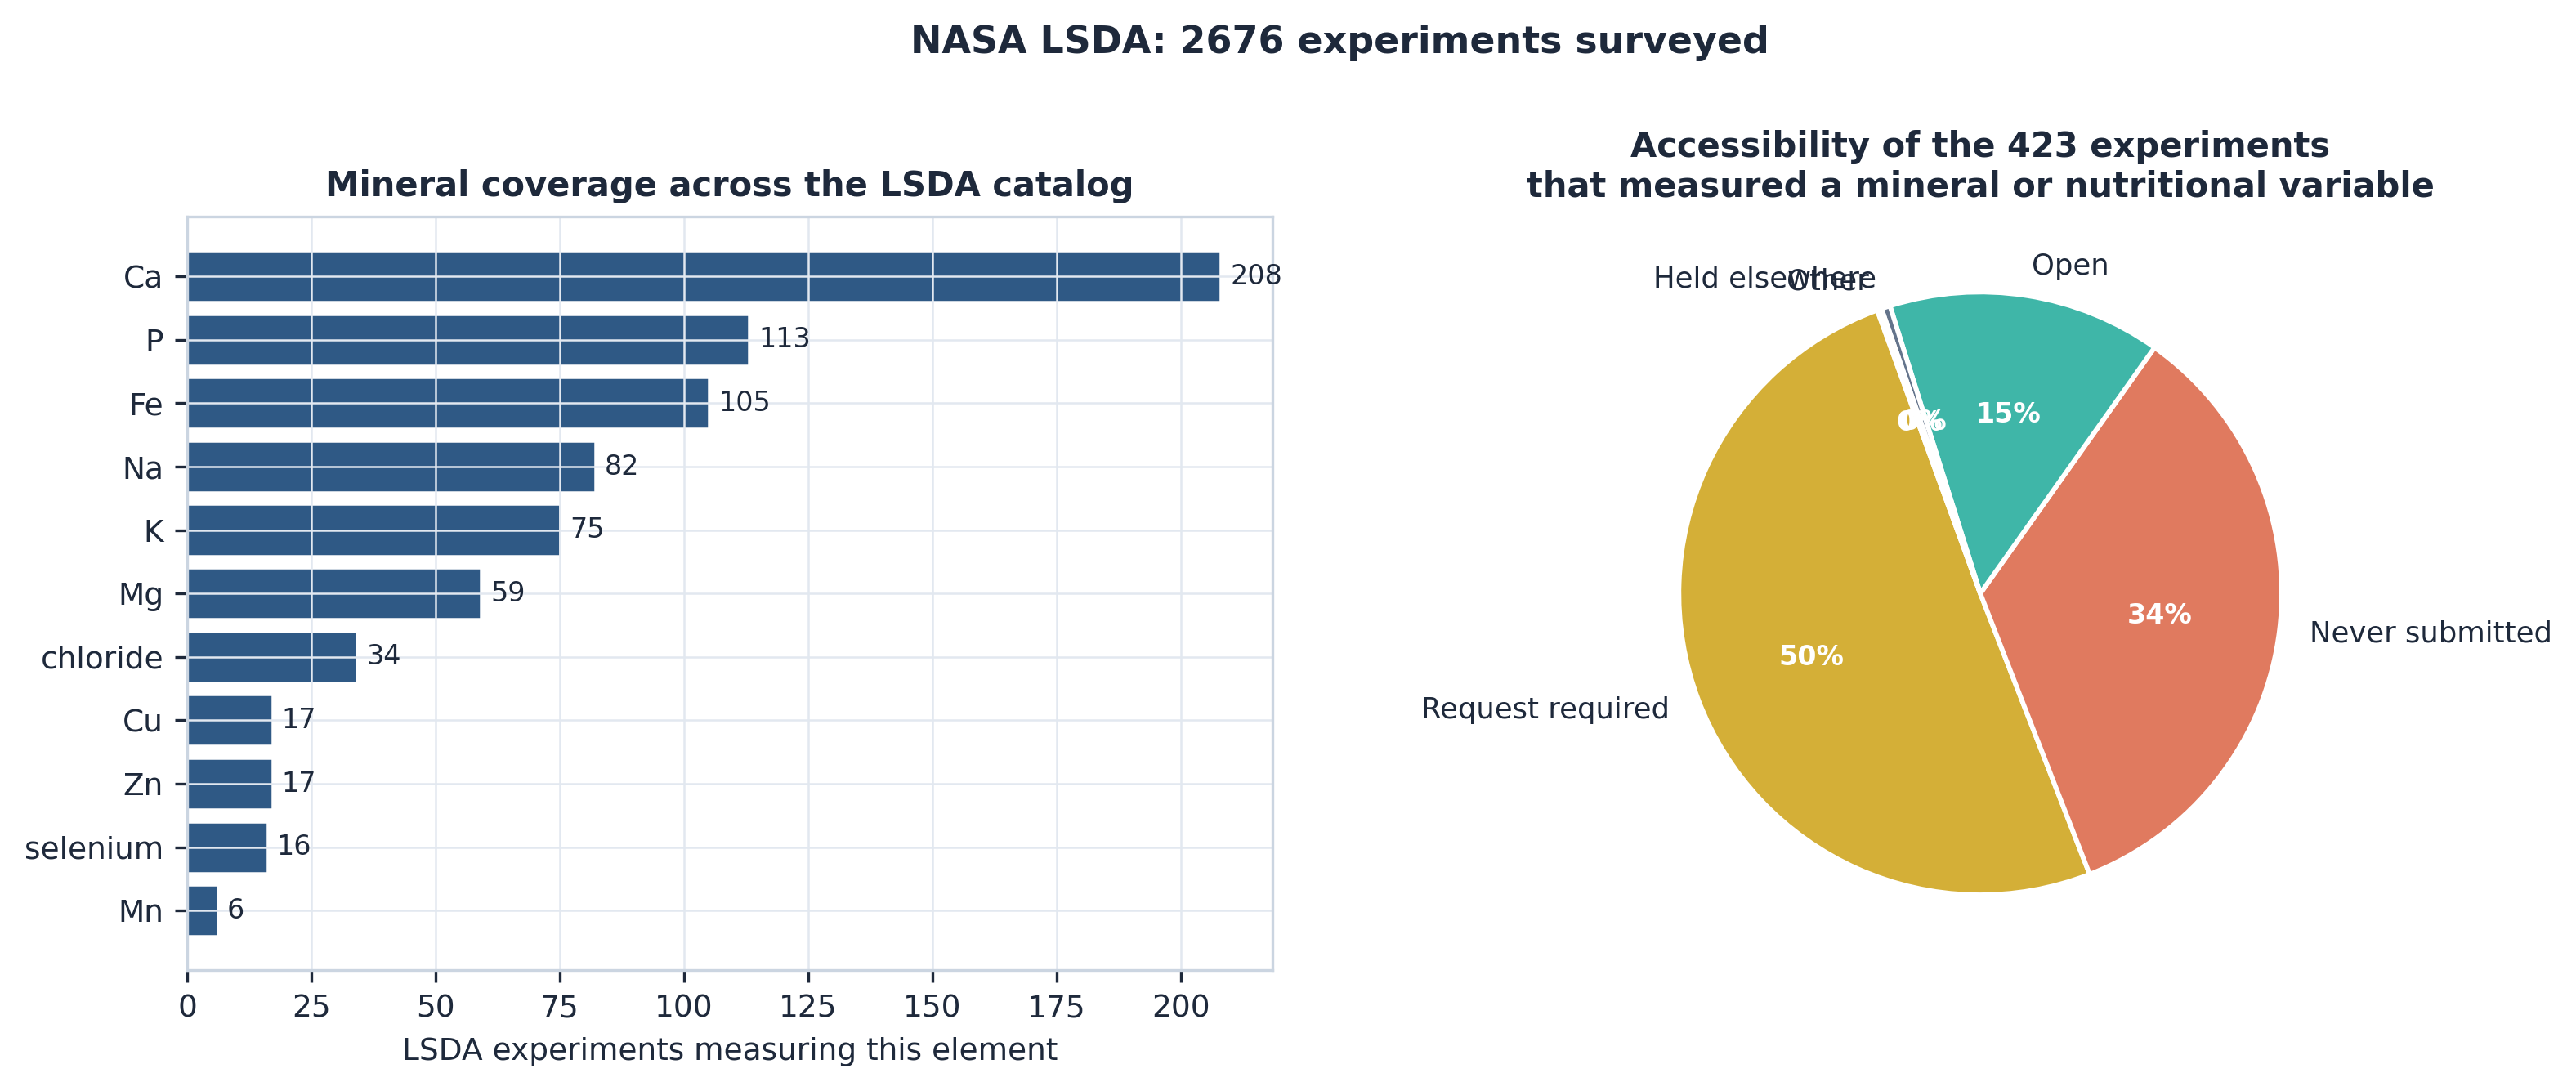
\includegraphics[width=\textwidth]{figures/fig7_lsda_landscape.png}
  \caption{Mineral and dietary data across the NASA Life Sciences Data Archive.
    Left: number of experiments measuring each element. Right: accessibility of
    the \LSDAMeasured{} experiments that measured a mineral or nutritional
    variable. Access, not measurement, is the binding constraint.}
  \label{fig:lsda}
\end{figure}

The survey identifies the Nutritional Status Assessment (SMO-016E) as the
highest-value target for this question: it measured ten minerals across
long-duration ISS missions with in-flight sampling, and underlies the
time-resolved analysis of \citet{zheng2023}. It is request-gated. Also
surfaced were the NASA Biochemical Profile Project, Food Physiology, and
Clinical Nutritional Assessment (MR016G), the last of which is openly
available.

\subsection{A unit-labelling defect inverts the cross-study comparison}

The OSD-655 elemental file and its archived data dictionary both label calcium,
potassium, magnesium, phosphorus and sulfur as mg/g dry weight. Taken at face
value, mean potassium is $2943\%$ of dry weight, magnesium $805\%$, calcium
$651\%$, sulfur $551\%$ and phosphorus $367\%$ --- each impossible.
Reinterpreted as $\mu$g/g, all five fall within the normal range for leafy
\emph{Brassica} tissue and agree with the independently-scaled OSD-745 lettuce
values. The six elements OSD-655 already labels in $\mu$g/g require no change
and agree across studies without correction, which localises the defect
precisely. \NUnitOverrides{} column corrections were applied, and all four
quality-control gates then passed.

The consequence is not cosmetic. Concatenating the two studies without this
correction places five of twelve elements on a scale 1000-fold larger in one
crop than the other, which would dominate any distance-based method, any
principal component analysis, and any model trained on the pooled data.

\subsection{The two crops diverge in their flight response}

At face value the two studies look very different. In lettuce, flight/ground
concentration ratios sit close to unity across the board --- calcium
\FcLetCa{}, potassium \FcLetK{}, iron \FcLetFe{} --- and no element reaches
significance. In Tokyo Bekana, eight elements rise together: sodium
\FcTbNa{}, sulfur \FcTbS{}, potassium \FcTbK{}, iron \FcTbFe{}, phosphorus
\FcTbP{}, boron \FcTbB{}, calcium \FcTbCa{} and magnesium \FcTbMg{}, with
\NSigConc{} significant at $q<0.05$.

A coordinated rise of that kind is the signature of a dry-matter dilution
effect rather than eight independent uptake changes, and the centred log-ratio
analysis separates the two (Figure~\ref{fig:clr}).

\begin{figure}[htbp]
  \centering
  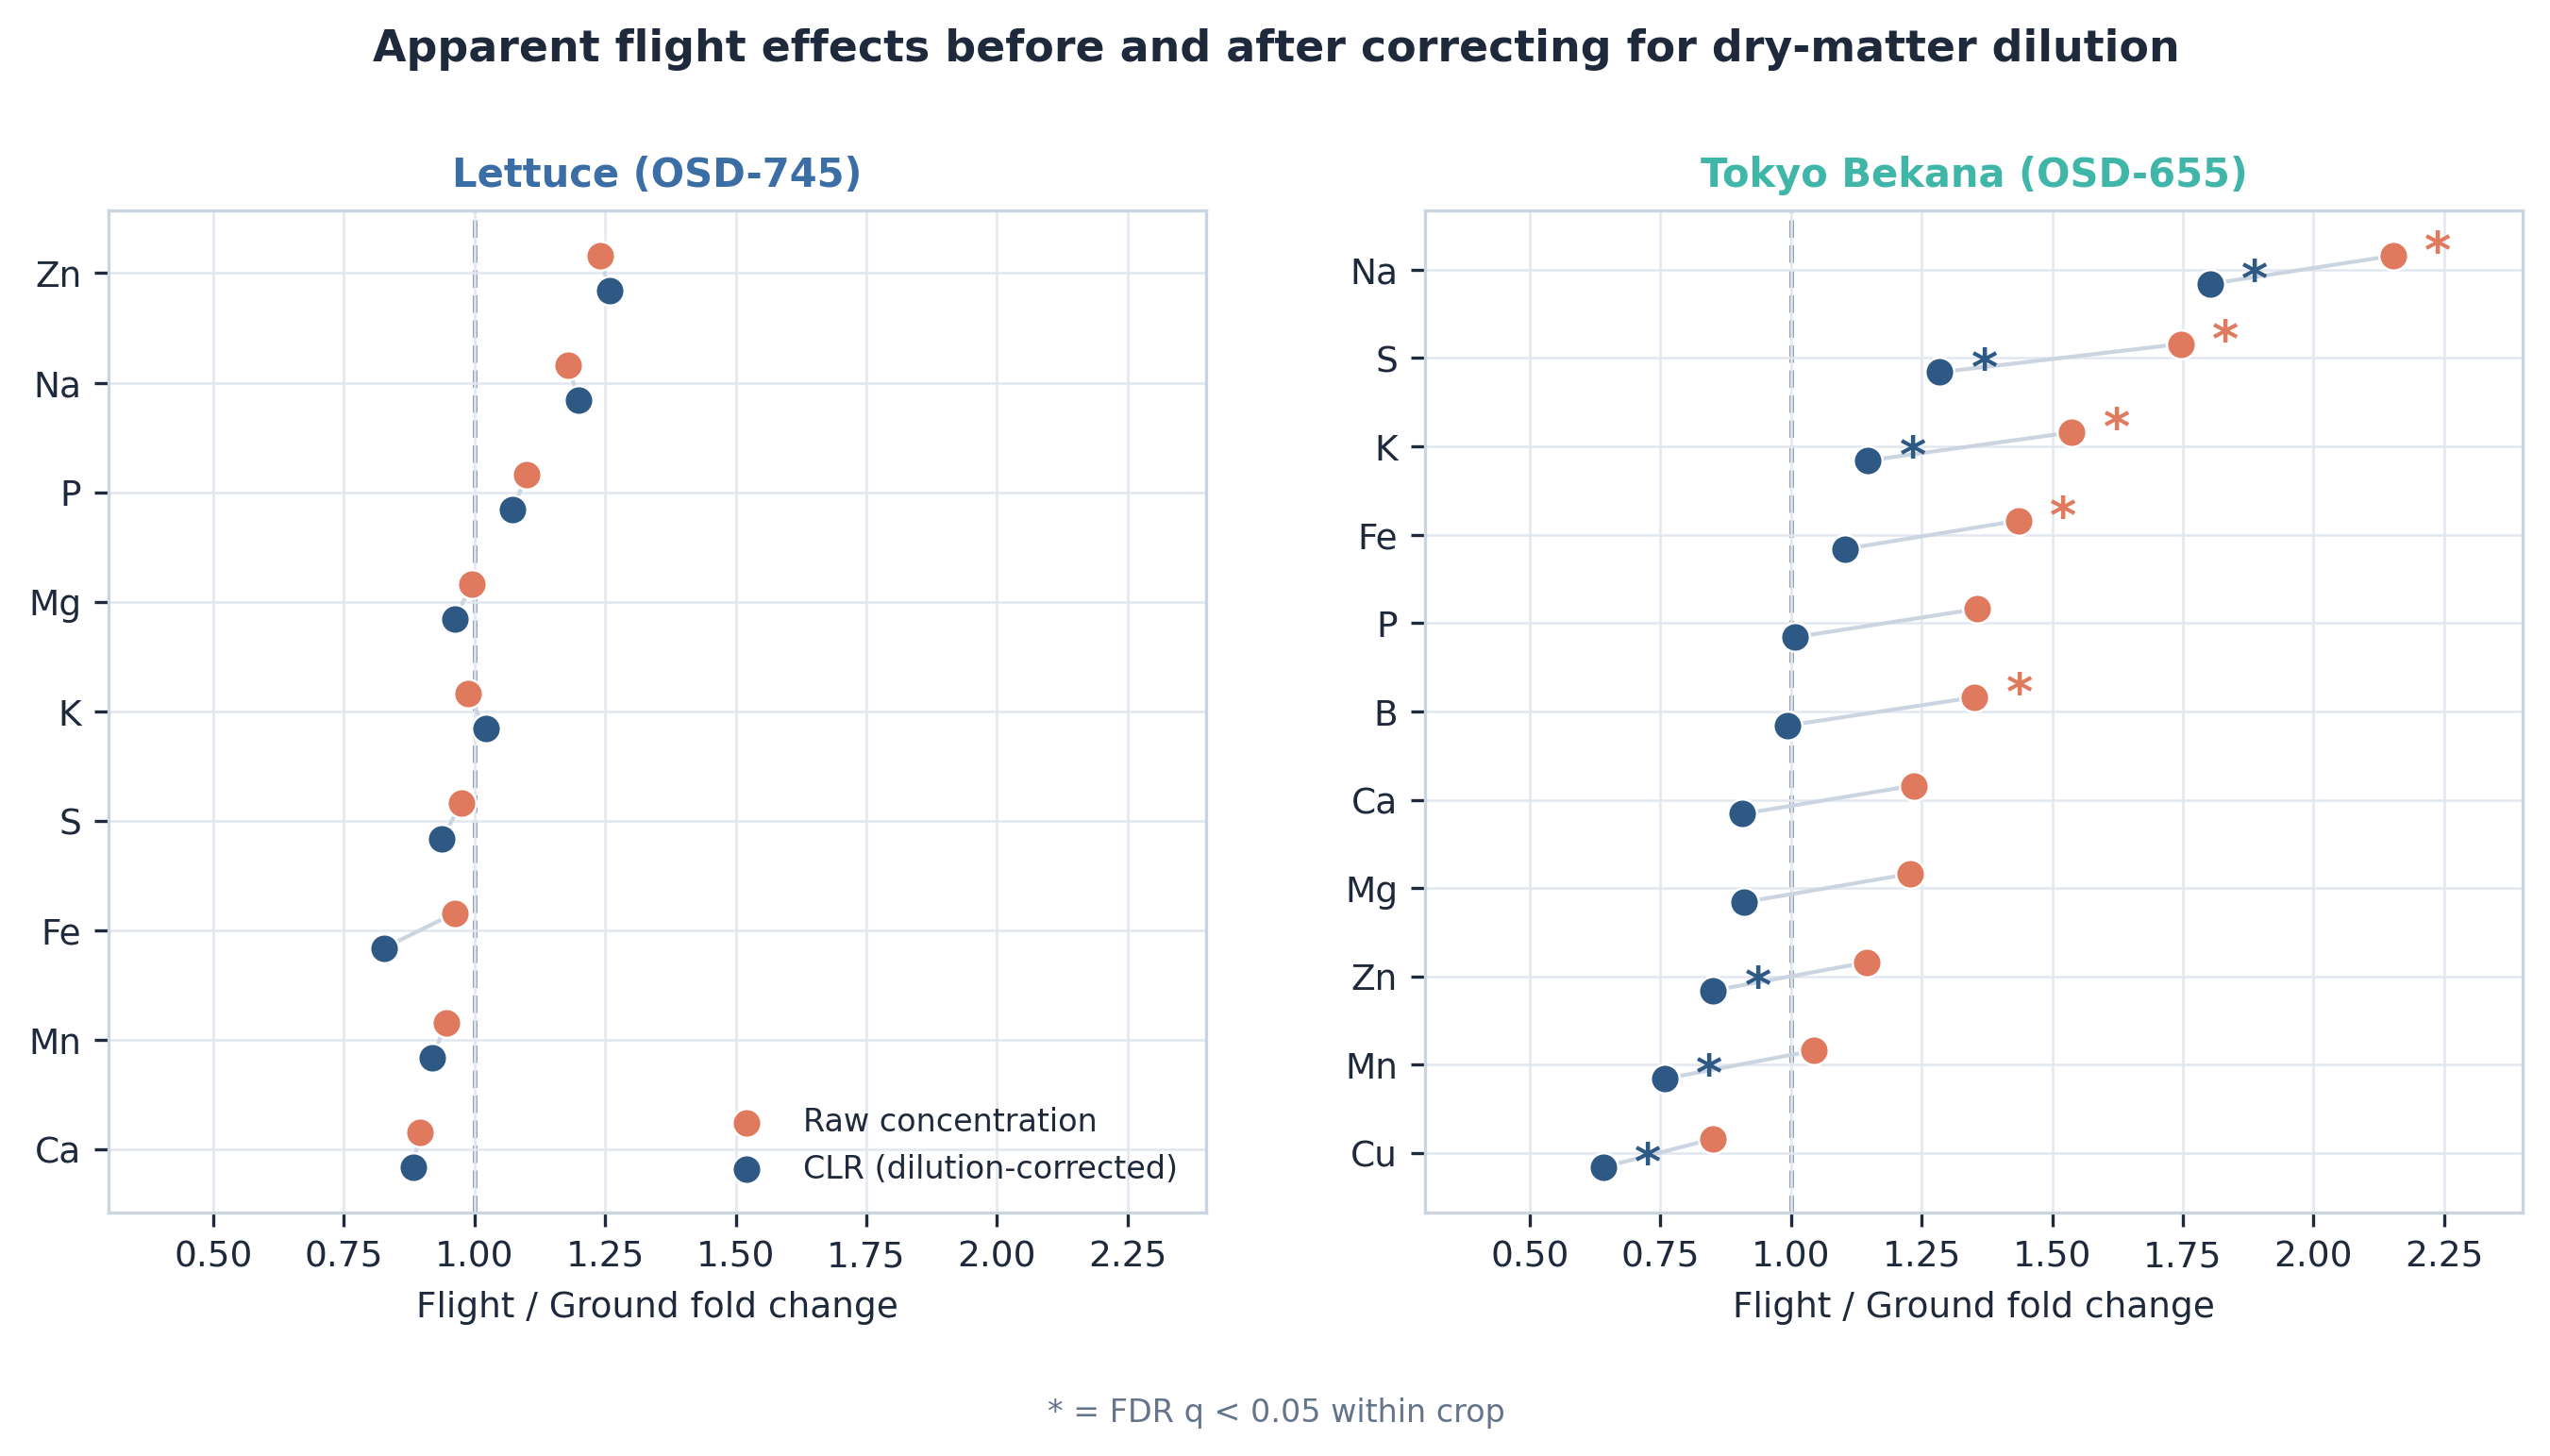
\includegraphics[width=\textwidth]{figures/fig1_fold_change_clr.png}
  \caption{Flight/ground fold changes before (coral) and after (navy)
    correcting for dry-matter dilution by centred log-ratio transform.
    Lettuce shows no significant change on either scale. In Tokyo Bekana the
    apparent calcium, magnesium, iron, boron and phosphorus increases collapse
    toward unity after correction, while sodium, sulfur and potassium persist.
    Asterisks mark $q<0.05$ within crop.}
  \label{fig:clr}
\end{figure}

After correction, \NSigCLR{} elements remain significant in Tokyo Bekana and
none in lettuce. Critically for the accumulation hypothesis that motivated this
work, the two divalent cations do not survive: calcium falls from \FcTbCa{} to
\FcclrTbCa{} ($q=\QclrTbCa$) and iron from \FcTbFe{} to \FcclrTbFe{}
($q=\QclrTbFe$). Both apparent increases are dilution artefacts. Potassium
persists (\FcTbK{} to \FcclrTbK{}, $q=\QclrTbK$), as do sodium (\FcclrTbNa)
and sulfur (\FcclrTbS). Copper, manganese and zinc become significantly
\emph{lower} in flight tissue once the composition is accounted for.

Only \NSigBoth{} elements --- potassium, sodium and sulfur --- are significant
on both scales, and these are monovalent cations and an anion, not the divalent
cations of the original hypothesis. Comparing the crops element by element
(Figure~\ref{fig:divergence}), \NDivergentCLR{} elements move in opposite
directions after correction (\DivergentElementsCLR).

\begin{figure}[htbp]
  \centering
  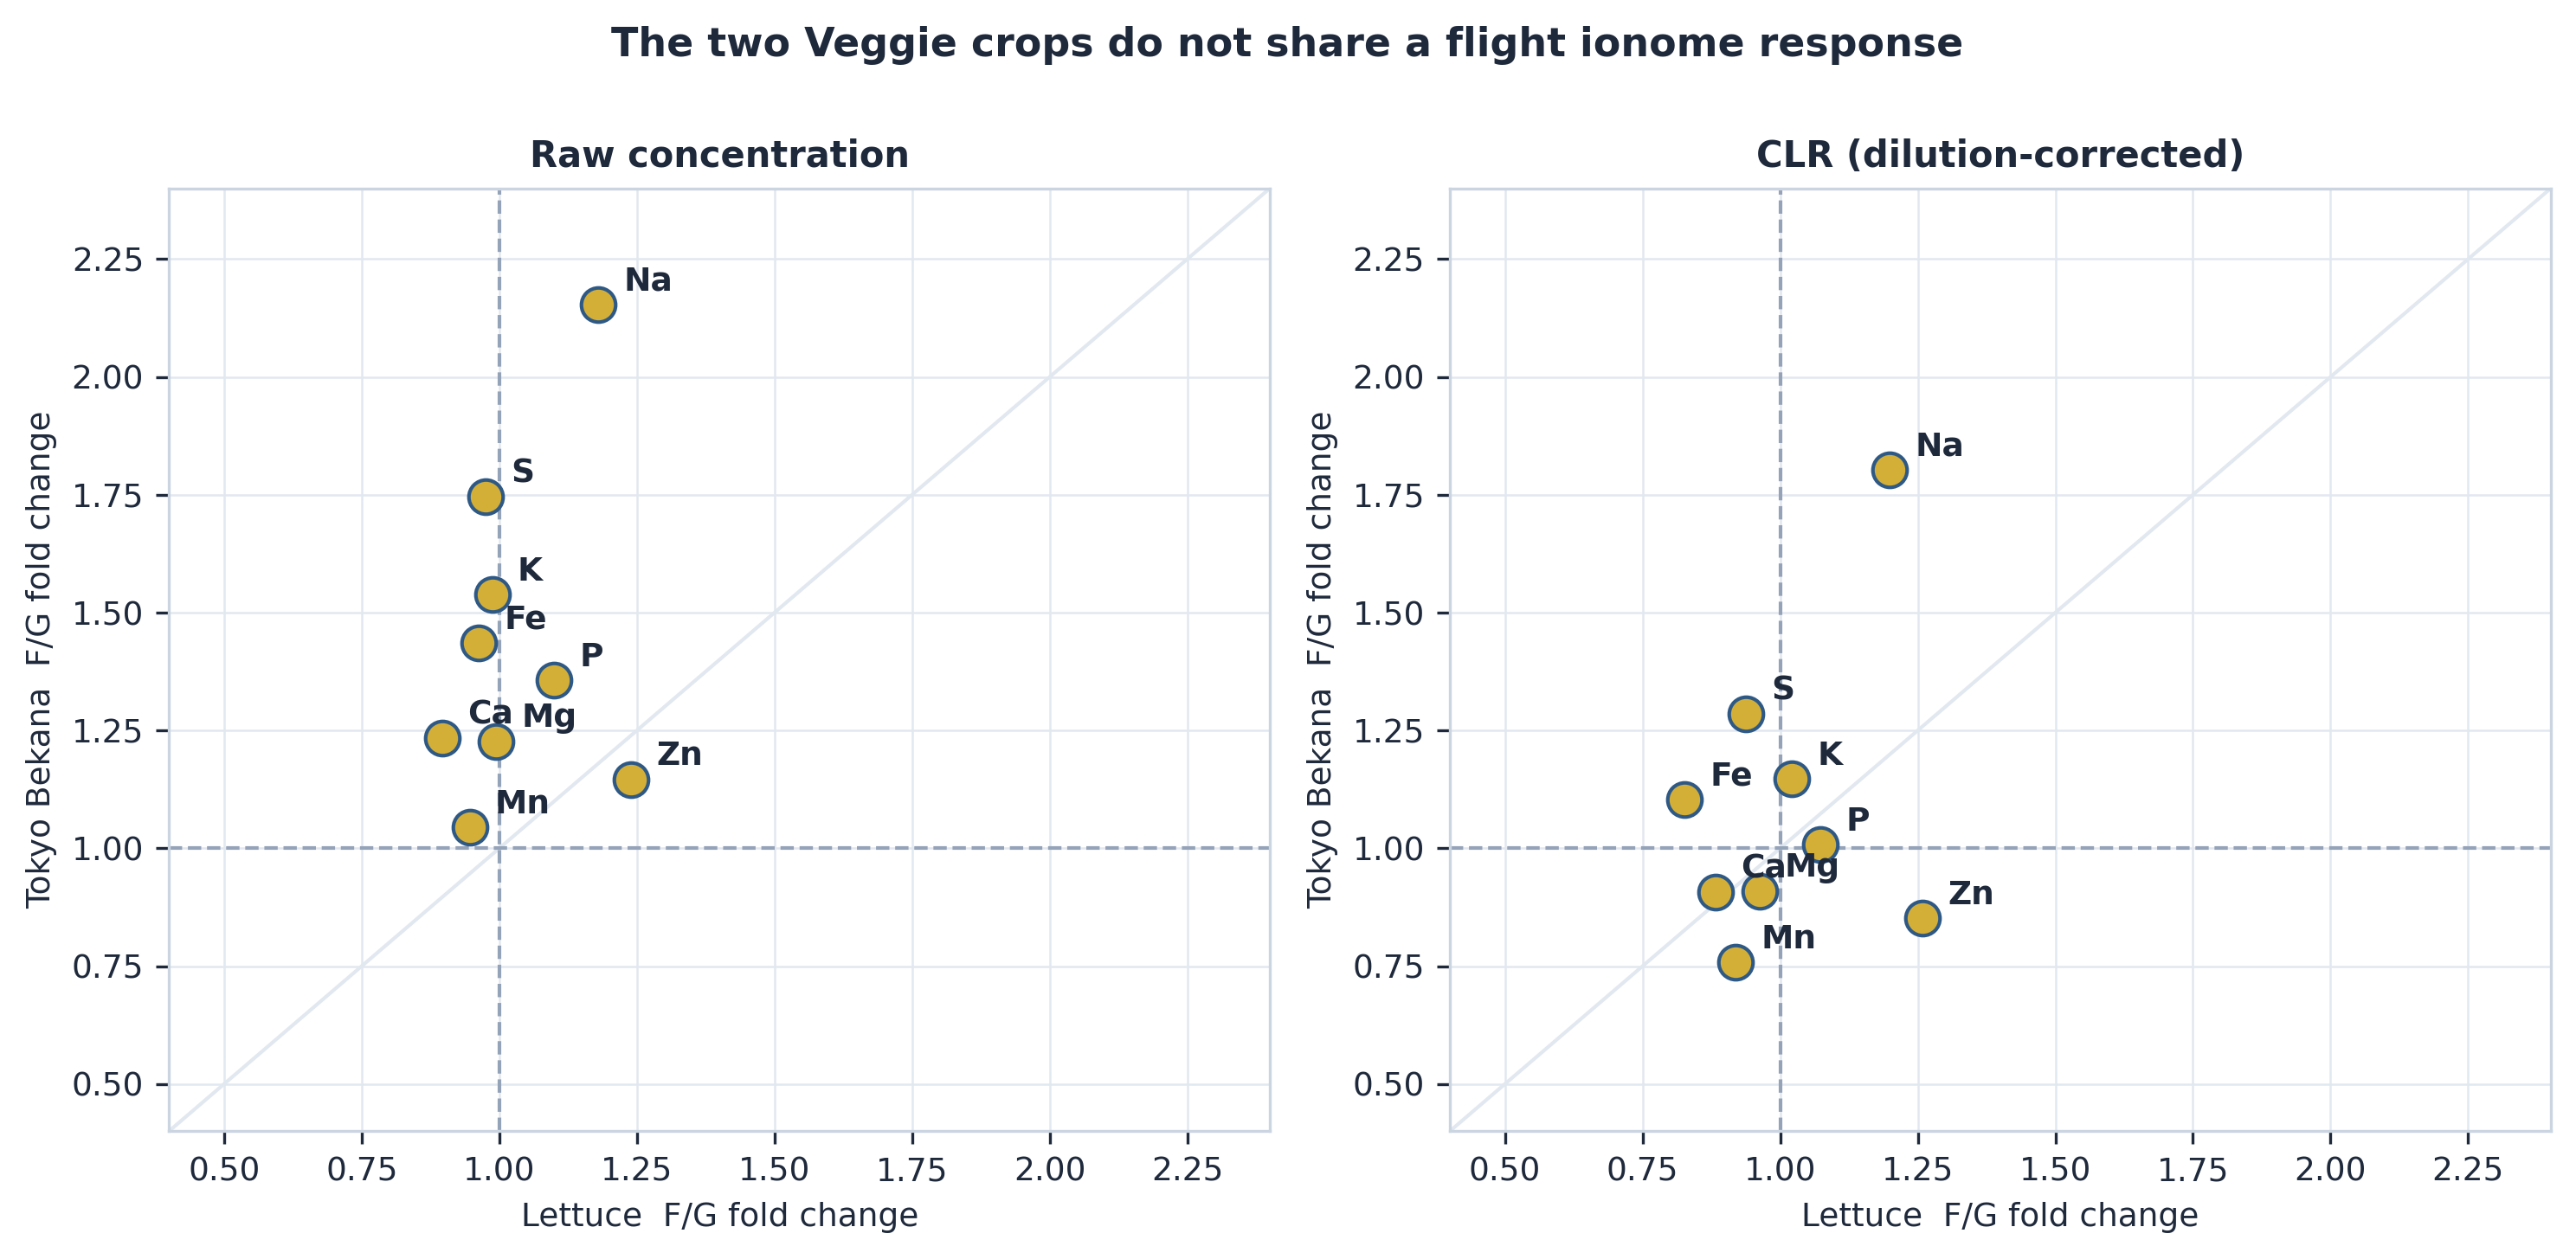
\includegraphics[width=\textwidth]{figures/fig2_crop_divergence.png}
  \caption{Lettuce versus Tokyo Bekana flight/ground fold change per element.
    Points on the diagonal would indicate a shared response. They do not lie on
    it on either scale.}
  \label{fig:divergence}
\end{figure}

\subsection{No flight signature transfers between crops}

Classification of flight versus ground from the ionome
(Figure~\ref{fig:ml}) confirms this from the opposite direction. Under
leave-one-mission-out cross-validation (\MlfoldsMission{} folds) the random
forest reaches \MlMissionRf{} balanced accuracy against a best baseline of
\MlbaselineMission{}, a margin of \MlMissionRfMargin{} with a 95\% confidence
interval of \MlMissionRfCi{} that spans chance. Penalised logistic regression
performs worse than baseline (\MlMissionLrMargin).

Under leave-one-crop-out --- training on one species and testing on the other
--- both models fall \emph{below} baseline (\MlCropRfMargin{} and
\MlCropLrMargin). A model that has learned the flight signature of one crop is
worse than useless on the other. That is not a failure of the method; it is a
direct measurement of the divergence, and it stands against previously reported
cross-species accuracies for this data that were not derived from any
implemented cross-species split.

\begin{figure}[htbp]
  \centering
  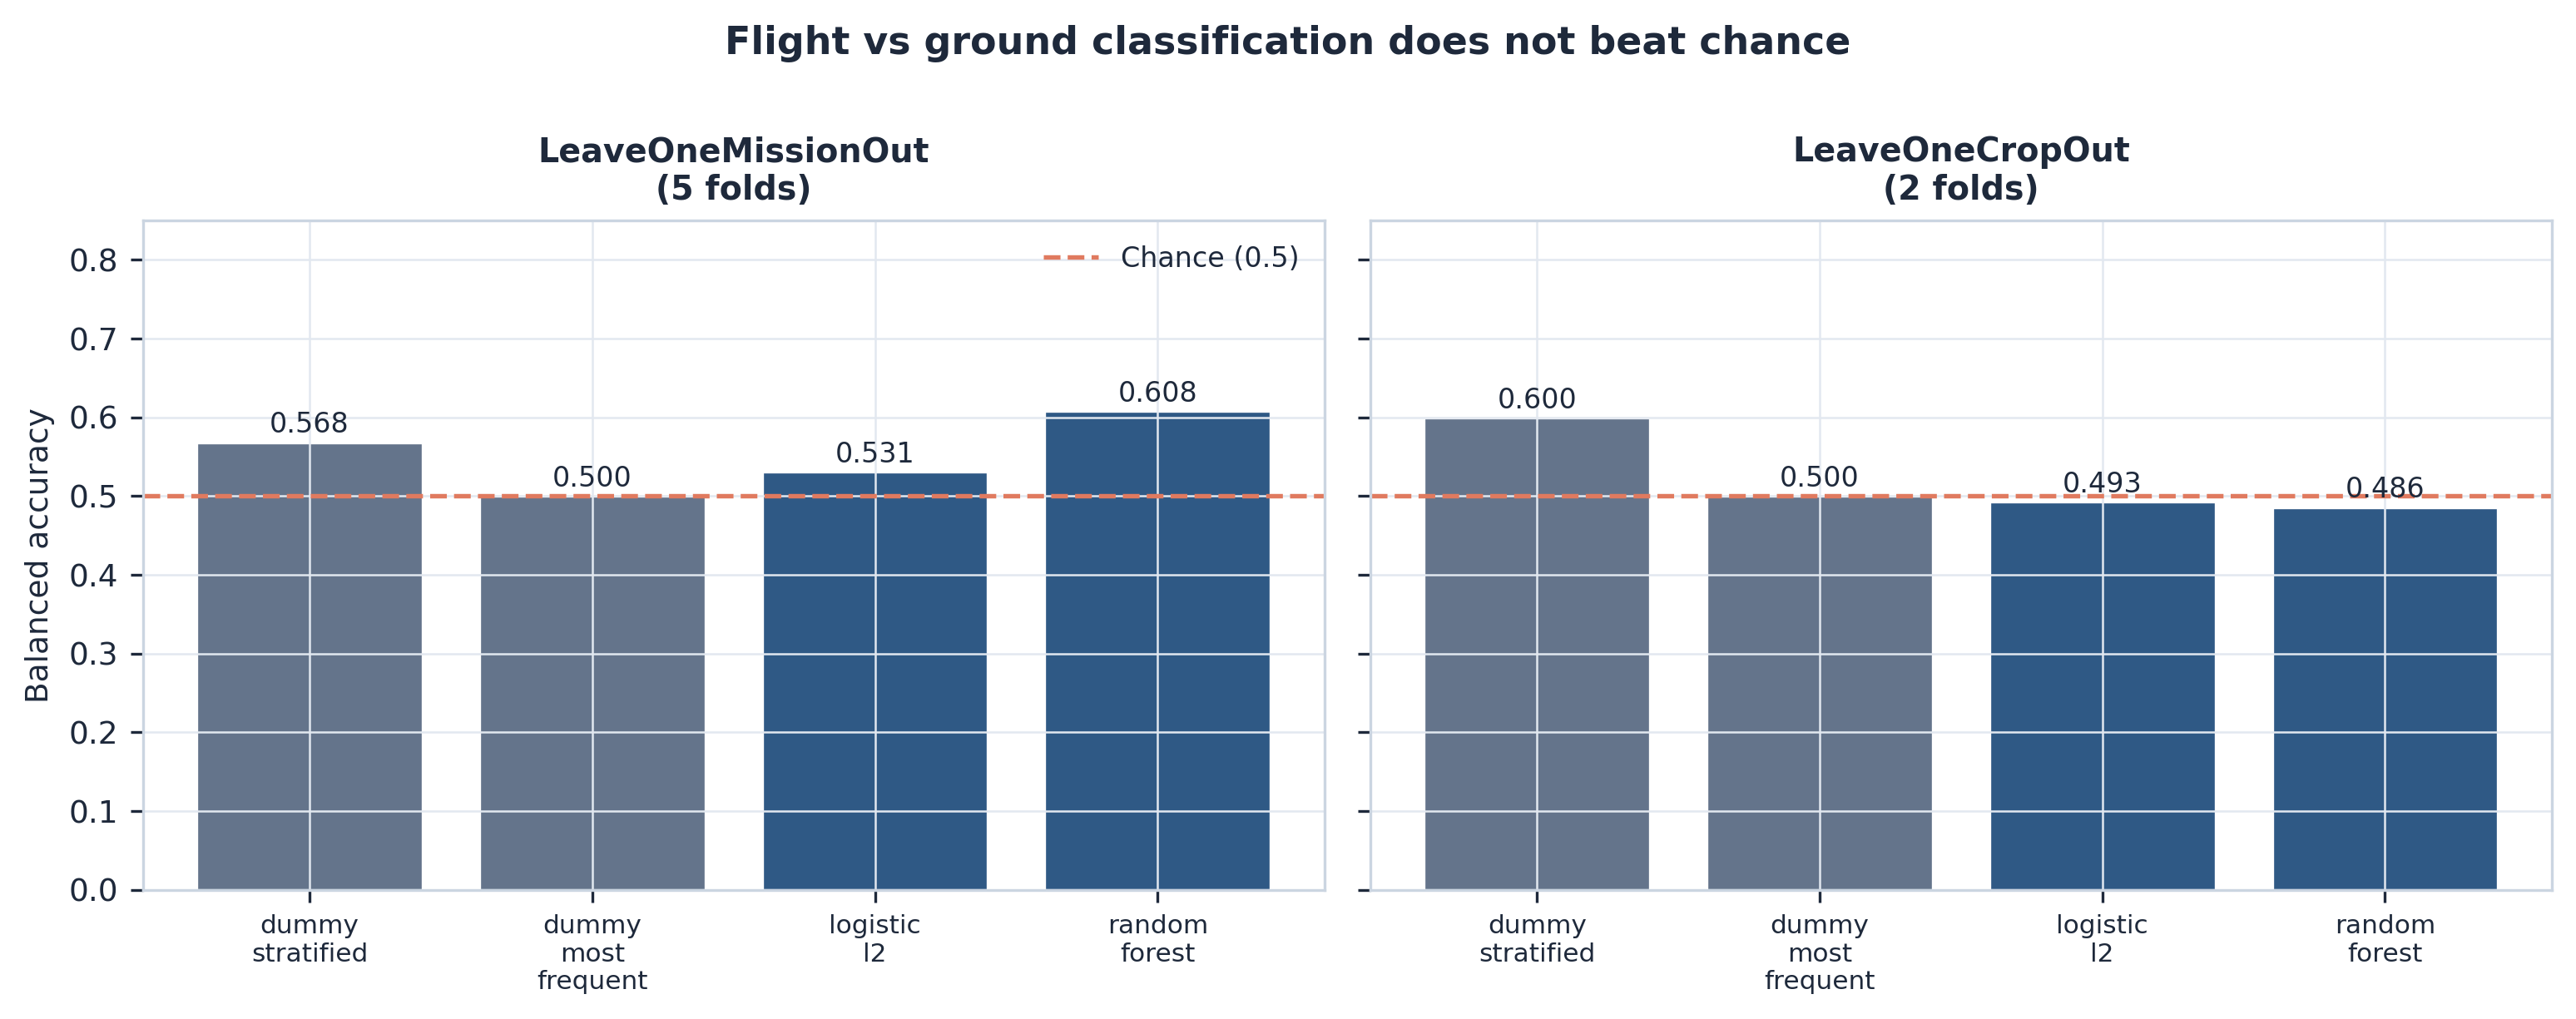
\includegraphics[width=0.92\textwidth]{figures/fig6_ml_performance.png}
  \caption{Balanced accuracy under both grouped cross-validation schemes,
    with the dummy baselines each model must beat.}
  \label{fig:ml}
\end{figure}

Permutation importance ranks \MltopOne, \MltopTwo{} and \MltopThree{} highest,
matching the three elements that survive compositional correction --- an
internal consistency between two methods that share no machinery.

\subsection{Astronaut serum minerals}

The Inspiration4 comprehensive metabolic panel provides \AstroObs{}
observations across \AstroN{} crew and \AstroTimepoints{} timepoints
(Figure~\ref{fig:serum}). Relative to each subject's pre-flight mean, potassium
fell in \AstrodownK{} of \AstroN{} crew at first return (median
\AstropctK\%), calcium in \AstrodownCa{} of \AstroN{} (median \AstropctCa\%),
and bicarbonate in \AstrodownCarbondioxide{} of \AstroN{}.

\begin{smacaution}[title=These data cannot establish a spaceflight effect]
Four subjects, a \AstroDuration-day mission, and no in-flight sample --- every
timepoint is pre-flight or post-return. The direction of change is reported
descriptively, per subject; no inferential test is appropriate at this size, and
none is performed.
\end{smacaution}

\begin{figure}[htbp]
  \centering
  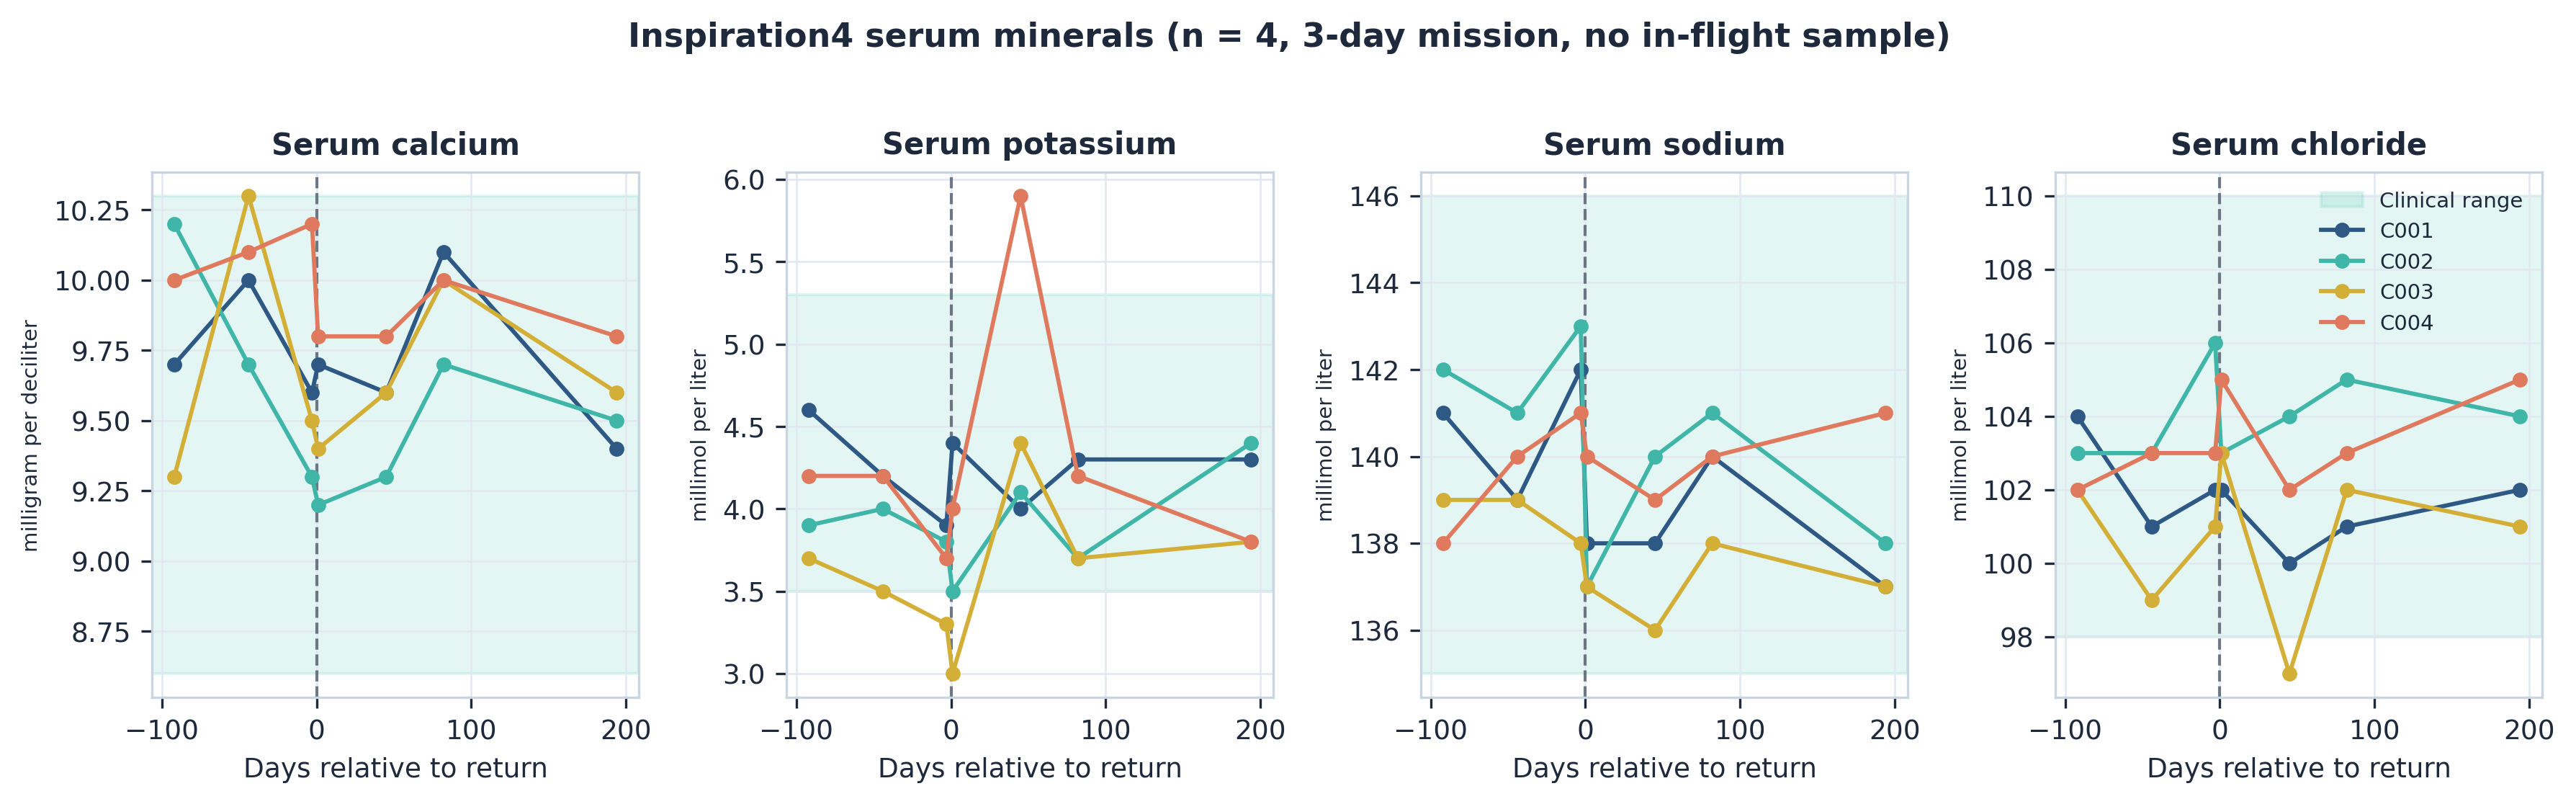
\includegraphics[width=\textwidth]{figures/fig4_astronaut_serum.png}
  \caption{Per-subject serum mineral trajectories, with the clinical reference
    range shaded. The dashed line marks return.}
  \label{fig:serum}
\end{figure}

\subsection{What a serving delivers, and whether overload is achievable}

Combining measured tissue concentrations with NASA daily requirements
\citep{jsc67378} gives the contribution of a realistic serving
(Figure~\ref{fig:serving}). A 100\,g fresh serving of flight-grown tissue at
$10\%$ dry matter supplies \ServeLetK\% (lettuce) and \ServeTbK\% (Tokyo
Bekana) of the daily potassium requirement, \ServeLetCa\% and \ServeTbCa\% of
calcium, and \ServeLetFe\% and \ServeTbFe\% of iron. Manganese is the standout:
a single serving supplies \ServeLetMn\% and \ServeTbMn\% of the daily
requirement.

\begin{figure}[htbp]
  \centering
  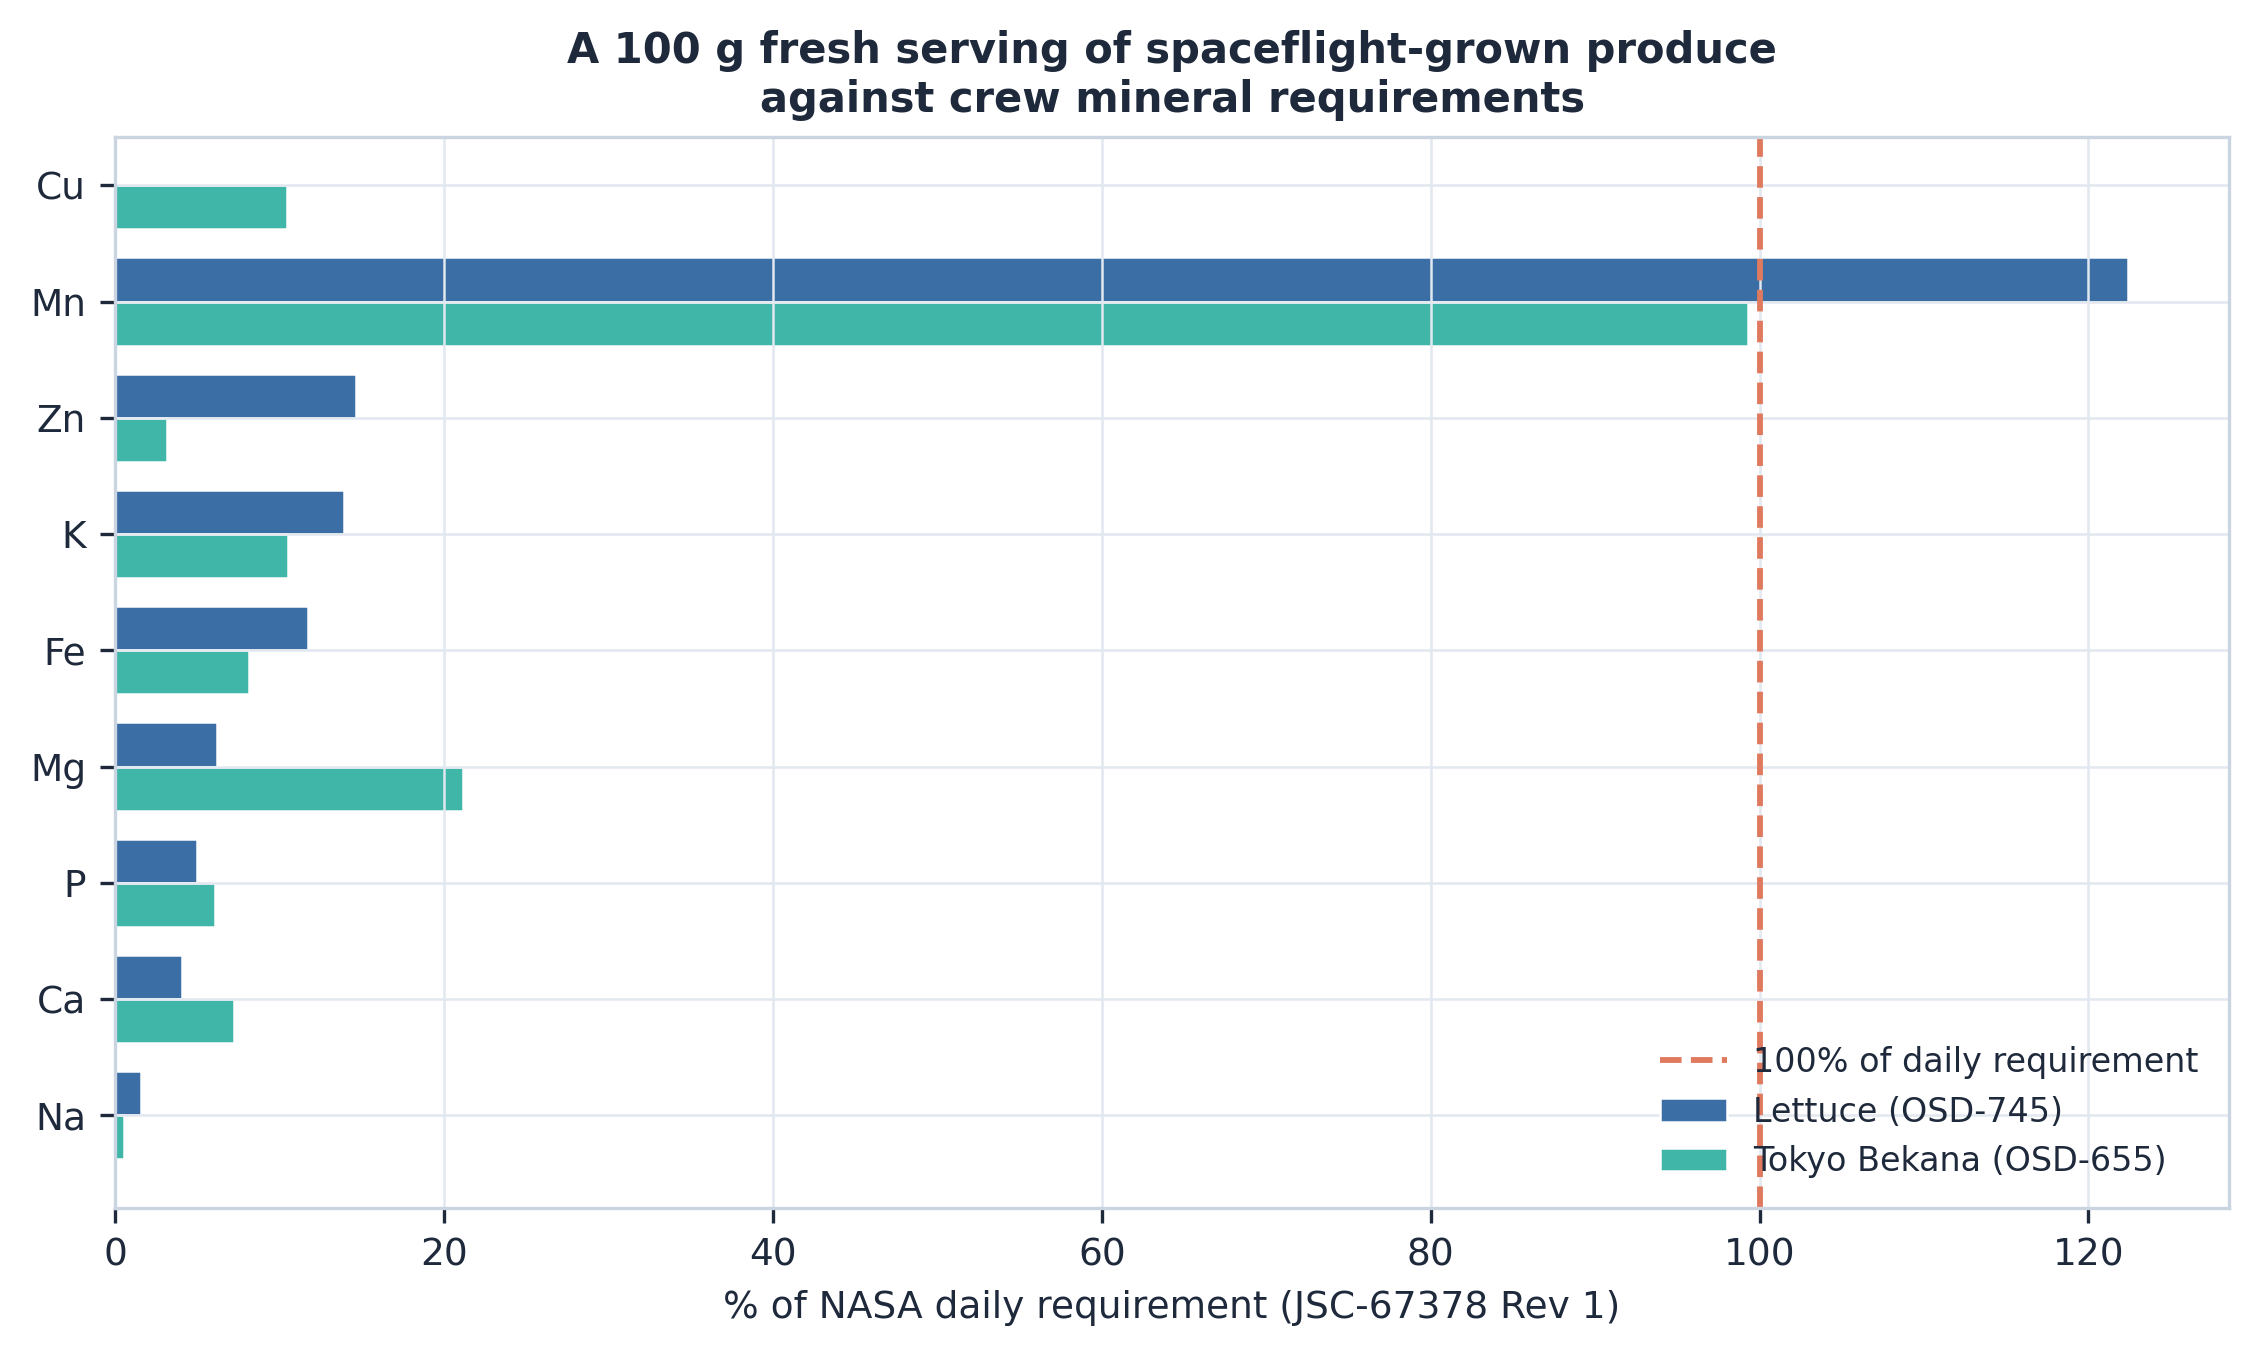
\includegraphics[width=0.88\textwidth]{figures/fig5_serving_contribution.png}
  \caption{Percentage of the NASA daily mineral requirement supplied by a
    100\,g fresh serving of flight-grown produce.}
  \label{fig:serving}
\end{figure}

The overload question can now be answered directly. Reaching NASA's iron upper
limit of 8\,mg/d would require \OverloadFeLet\,kg of fresh lettuce or
\OverloadFeTb\,kg of Tokyo Bekana per day; the zinc limit of 40\,mg/d would
require \OverloadZnLet\,kg and \OverloadZnTb\,kg respectively. A VEG-04A pillow
produced roughly \BiomassFlight\,g fresh, so the iron limit alone would demand
the entire yield of more than twenty pillows daily. Dietary mineral overload
from Veggie produce is not achievable at any plausible harvest scale.

\subsection{Supply-normalised uptake}

Per-pillow water delivery and harvest mass were recovered for \SupplyMatched{}
of \SupplyTotal{} Tokyo Bekana samples (VEG-04A only). Flight pillows received
less water than ground controls (\WaterFlight{} versus \WaterGround\,mL) while
producing comparable biomass (\BiomassFlight{} versus \BiomassGround\,g),
giving a higher apparent water-use efficiency in flight
(\WueFlight{} versus \WueGround\,g fresh mass per litre). Because no dry-matter
fraction is archived, absolute uptake efficiency cannot be computed; the
implications are taken up in Section~\ref{sec:discussion}.

\section{Discussion}
\label{sec:discussion}

\subsection{Crop-specific responses argue against a general spaceflight ionome}

The clearest result is negative in a useful way: there is no shared
flight-induced ionome response across the two Veggie crops with archived
elemental data. Lettuce shows no significant change in any element on either
scale; Tokyo Bekana shows \NSigCLR{} after compositional correction, and
\NDivergentCLR{} elements move in opposite directions between the crops. A
classifier trained on one crop performs below chance on the other.

This matters for how spaceflight crop nutrition is generalised. Statements of
the form ``spaceflight increases mineral $X$ in leafy greens'' are not supported
by these data even across two leafy green species grown in the same hardware.
The two studies differ in more than species --- mission, duration, light
spectrum, harvest protocol --- and those covariates cannot be separated with
$n=\NSamples$. That is precisely the point: with the available data, crop
identity and its confounds cannot be disentangled, so a species-general claim is
not currently derivable from the archive.

\subsection{Compositional artefacts are the dominant failure mode}

The apparent calcium and iron increases in Tokyo Bekana --- \FcTbCa$\times$ and
\FcTbFe$\times$, both large and one significant --- do not survive correction
for dry-matter dilution. Had we reported the raw concentrations, we would have
reported an accumulation effect that the data do not support.

This is a general hazard for ICP-OES tissue data, which is compositional by
construction \citep{aitchison1982}. Any treatment that changes tissue water
content, structural carbohydrate or non-mineral dry matter shifts every
concentration together. Spaceflight plausibly does all three. We would suggest
that reporting a concentration fold change without a compositional or
content-based check should be treated as an incomplete analysis in this
literature, not a stylistic preference.

The elements that survive are informative in their own right. Potassium, sodium
and sulfur are the mobile ions most closely tied to water relations and
osmotic adjustment, which is a coherent picture for plants in altered
root-zone water distribution --- and consistent with the reduced water delivery
recorded for flight pillows.

\subsection{Data quality is a first-order scientific problem}

The OSD-655 unit defect is a 1000-fold error on five of twelve elements, present
in both the data files and the archived data dictionary, in an openly available
and citable NASA dataset. It is not hidden --- a plausibility check catches it
immediately --- but nothing in the archive's own metadata flags it, and a
pipeline that trusts the stated unit inherits it silently.

We have written this up for the OSDR curation team
(\path{fair/osdr_curation_report.md}). The broader lesson is that a FAIR
dataset is interoperable only to the extent its unit metadata is correct, and
that automated plausibility gates belong in analysis pipelines as a matter of
routine. The gate that caught this is four lines of arithmetic.

\subsection{Overload is not the risk; sufficiency is the question}

The concern that motivated this work --- that plant-rich diets combined with
spaceflight-altered mineral handling could drive crew mineral overload --- is
not supported. Reaching NASA's iron upper limit would require
\OverloadFeLet\,kg of fresh lettuce daily, against a per-pillow yield of
roughly \BiomassFlight\,g. The margin is two orders of magnitude.

The useful question is the opposite one. A 100\,g serving supplies
\ServeLetK\% of daily potassium and \ServeLetCa\% of daily calcium: real but
supplementary contributions. The exception is manganese, at \ServeLetMn\% of
the daily requirement from a single serving, which is worth monitoring as
Veggie-type production scales --- not because these values approach a toxic
threshold, but because it is the one element where produce could plausibly
become a dominant dietary source.

\subsection{The missing measurements}

Two absences constrain everything above, and both are cheap to fix.

\emph{Dry-matter fraction.} OSD-655 archives fresh harvest mass and per-dry-gram
concentrations but no dry-matter fraction, so total mineral content per plant
cannot be computed and uptake efficiency is unavailable. Dry-matter fraction is
routinely measured during ICP-OES sample preparation --- the tissue must be
dried to be analysed. Archiving that number would convert a bounded estimate
into a measurement, and would also allow the dilution correction of
Section~\ref{sec:clr} to be tested directly rather than inferred.

\emph{Substrate elemental composition.} No Veggie study archives the elemental
composition of the arcillite substrate and its controlled-release fertiliser
charge. Without it, bioavailability --- the fraction of supplied mineral that
reaches edible tissue --- cannot be computed at all. Our water-normalised index
is a proxy for the mass-flow driver, not a bioavailability fraction, and we
name it accordingly.

\subsection{What the crew-side data can and cannot support}

The Inspiration4 panel gives real, openly available serum mineral measurements,
and the post-flight potassium decline in \AstrodownK{} of \AstroN{} crew is a
genuine observation. But four subjects on a \AstroDuration-day mission with no
in-flight sampling cannot establish a spaceflight effect, and the plant and crew
data describe different missions and different people.

The dataset that would close this loop exists: the Nutritional Status
Assessment (SMO-016E), with 27 astronauts across long-duration ISS missions,
in-flight sampling, and paired dietary intake and serum chemistry
\citep{zheng2023}. Our LSDA survey confirms it is request-gated rather than
open. Section~\ref{sec:availability} and the request package in
\path{lsda_request/} set out the route.

\subsection{Limitations}

\begin{itemize}\itemsep2pt
  \item $n=\NSamples$ plant samples in total (\NLet{} lettuce, \NTb{} Tokyo
        Bekana). The crop divergence needs replication before it is treated as
        established.
  \item Crop, mission, duration and light spectrum are confounded; the
        divergence is between studies, not cleanly between species.
  \item The compositional correction assumes the dilution factor is
        multiplicative and shared across elements within a sample. Direct
        dry-matter measurement would test this.
  \item Water and mass supplements cover VEG-04A only
        (\SupplyMatched/\SupplyTotal{} samples), and biomass is fresh weight.
  \item Serving calculations assume a $5$--$10\%$ dry-matter fraction from the
        literature, not from these studies.
  \item The astronaut cohort is $n=\AstroN$ over \AstroDuration{} days with no
        in-flight sample.
  \item LSDA annotation is text-matching over catalog metadata; an experiment
        whose record does not name its analytes will be missed, so
        \LSDAMeasured{} is a lower bound.
\end{itemize}

\section{Conclusion}

Spaceflight does not act on the plant ionome in a way that generalises across
the two Veggie crops with archived elemental data. Lettuce shows no significant
change in any of ten elements; Tokyo Bekana shows \NSigCLR{} once dry-matter
dilution is accounted for, and a classifier trained on either crop fails on the
other. Apparent calcium and iron increases --- the specific accumulation
hypothesis this work set out to test --- are dilution artefacts and do not
survive compositional correction. Potassium, sodium and sulfur do.

Two contributions are methodological rather than biological, and may matter
more. A 1000-fold unit-labelling defect in OSD-655, present in the archived
data dictionary as well as the data files, would corrupt any pooled analysis
that trusted the stated units; it is caught by a plausibility gate that any
pipeline could run. And treating ICP-OES concentrations as compositional rather
than independent changes the conclusion for five of twelve elements.

On the question that motivated the work, dietary mineral overload from
spaceflight-grown produce is not achievable at plausible harvest scales ---
\OverloadFeLet\,kg of fresh tissue daily would be needed to reach the iron
limit. Sufficiency, not excess, is the operative question, and manganese is the
element to watch.

Progress now depends on access rather than analysis. Of \LSDAMeasured{} LSDA
experiments measuring a mineral or nutritional variable, \LsdaaccessOpen{} are
open and \LsdaaccessRequestrequired{} are request-gated. Two inexpensive
additions to future crop studies --- archived dry-matter fraction and substrate
elemental composition --- would convert several of this study's bounded
estimates into measurements.

\section{Data and code availability}
\label{sec:availability}

\subsection{Data used in this study}

All plant and crew data are openly available from the NASA Open Science Data
Repository and were retrieved programmatically:
OSD-745 \citep{osdr745}, OSD-655 \citep{osdr655} and OSD-575 \citep{osdr575}.
SHA-256 digests of every retrieved file are recorded in
\path{fair/checksums.sha256}. The LSDA experiment catalog \citep{lsda} was
harvested from the public JSON query endpoint; the annotated catalog is
released with this work as \path{catalog/lsda_mineral_nutrition_catalog.csv}.

\subsection{Data not openly available}

The Nutritional Status Assessment (SMO-016E) and Validation of Procedures for
Monitoring Crewmember Immune Function (SMO-015), which together underlie
\citet{zheng2023}, are held by the NASA Life Sciences Data Archive and are not
openly downloadable. LSDA directs requests to
\url{https://nlsp.nasa.gov/explore/lsdahome/datarequest}. A prepared request
covering the variables required to extend this analysis --- paired dietary
intake and serum mineral concentrations across pre-flight, in-flight and
post-flight timepoints --- is included in \path{lsda_request/}, together with
the schema and the loader function into which those data would be ingested
without modification to the analysis.

\subsection{Code}

The complete pipeline is released under the MIT licence; text, figures and
derived data tables under CC BY 4.0. The analysis runs end to end with
\texttt{make all}. An RO-Crate manifest, data dictionary and Zenodo deposition
metadata are in \path{fair/}.

\subsection{Note on a prior analysis of these studies}

An earlier dashboard and manuscript covering OSD-745, OSD-655 and OSD-780
reported flight/ground effects, model accuracies and cross-species
generalisation for these studies. Those values were generated by a synthetic
data routine rather than measured, and are not comparable with the results
reported here. A correction note and a working replacement data-acquisition
module are provided in \path{veggie_correction/}. We record this here because
the affected figures have been publicly posted, and readers comparing the two
should know which rests on measurements.


\bibliographystyle{unsrtnat}
\bibliography{references}

\end{document}
